% Inizio; comandi generali
\documentclass[a4paper, 11pt]{article}

% Pacchetti per il supporto multilingue
\usepackage[utf8]{inputenc} % Per la codifica UTF-8
\usepackage[T1]{fontenc} % Per font corretti con caratteri accentati
\usepackage[italian]{babel} % Per la lingua italiana

% Font e gestione dei caratteri
\usepackage{lmodern} % Font Latin Modern scalabile
\renewcommand{\familydefault}{\rmdefault} % Font roman come predefinito
\usepackage{setspace} % Per il controllo dell'interlinea
\setstretch{1} % Interlinea di 1.0

\usepackage{microtype}

% Matematica
\usepackage{amsmath} % Estensioni matematiche
\usepackage{amssymb} % Simboli aggiuntivi
\usepackage{textgreek} % Per lettere greche in modalità testo

\usepackage{tikz}
\usetikzlibrary{trees}

% Grafica e immagini
\usepackage{graphicx} % Per includere immagini
\usepackage{float} % Per posizionamento accurato degli oggetti flottanti

% Margini e layout della pagina
\usepackage[left=2cm, right=2cm, top=2cm, bottom=2cm]{geometry} % Margini personalizzati

% Titoli delle sezioni e struttura del documento
\usepackage{titlesec} % Per personalizzare lo stile dei titoli
\titleformat{\paragraph}[runin]
  {\normalfont\normalsize\bfseries}{\theparagraph}{0.5em}{}
\titlespacing*{\paragraph}{2pt}{0.5em}{0.5em}

% Controllo dell'indentazione del paragrafo
\setlength{\parindent}{0pt} % Nessuna indentazione della prima riga di ogni paragrafo

% Gestione avanzata dei font
\usepackage{fix-cm} % Per dimensioni flessibili dei font

% Fine preambolo; inizia il documento


\begin{document}

    % Frontespizio
    \begin{titlepage}
        \centering
    
        % Titolo
        \vspace{2cm}
        {\Huge\bfseries Algoritmi di ottimizzazione\par}
    
        % Autore
        \vspace{1cm}
        {\Large\itshape Appunti di Morello Filippo\par}
    
        % Data
        \vfill
        {\large II semestre 2025\par}
    
    \end{titlepage}

    % Sommario
    \tableofcontents

    \break
    
    \section{Introduzione}
        \subsection{Esempi introduttivi}
            \subsubsection*{La compilation ideale}
            Si vuole realizzare una compilation ideale avendo disposizione dei file musicali e un CD-ROM dalla capacità di $800$ MB. l’indice di
            gradimento (in una scala da 1 a 10) e l’ingombro in MB di ogni file sono riportati nella tabella seguente: 

            \begin{table}[ht]
                \centering
                \begin{tabular}{|c|c|c|c|}
                \hline
                \textbf{Canzone} & \textbf{Gradimento} & \textbf{Ingombro} \\ \hline
                Light my fire    & 8.0                 & 210               \\
                Fame             & 7.0                 & 190               \\
                I will survive   & 8.5                 & 235               \\
                Imagine          & 9.0                 & 250               \\
                Let it be        & 7.5                 & 200               \\
                I feel good      & 8.0                 & 220               \\ \hline
                \end{tabular}
                \end{table}
           

            \paragraph{Obiettivo: } Si vuole decidere quali file inserire nel CD in modo tale da massimizzare il gradimento complessivo senza eccedere la capacità del CD

            \paragraph{Soluzione: } Il problema può essere modellato per mezzo di variabili decisionali binarie associate a ogni file musicale in modo tale che assumono valore uno se il file in questione e inserito nel CD valore zero in caso contrario.

            Indicato con gi il gradimento della canzone i-esima, con wi il suo ingombro e con C la capacità del CD il problema può essere formulato per mezzo del seguente problema PLI: 

            Quindi:



            \[
                x_i = 
                \begin{cases}
                    1 \text{ se la cancone i-esima è inserita nel CD} \\
                    0 \text{ altriemnti}
                \end{cases}
            \]

            
            \textbf{CONSTRAINTS: }
            
            
            \[
                210x_1+190x_2+\ldots+220x_6 \leq 800
            \]
            


            \textbf{funzione di gradimento: }
            


            \[
                \max_{x} z = 8x_1 + 7x_2+\ldots+8x_6
            \]


            Scritto in modo più compatto:
            
            \begin{align}
                \max_{x} z &= \sum_{i = 1}^{n = 6} g_ix_i \notag \\
                \sum_{i = 1}^{n = 6} w_ix_i &\leq C = 800 \notag \\
                x_i &\in {0,1}, \text{ $\forall$ } i = 1,\ldots, n (= 6 )  \notag
            \end{align}



            dove n = 6 è ilnumero di file musicali. L’unico vincolo del problema consiste nel fatto che l’ingombro dei file inseriti non deve eccedere la capacità del CD.

            \textbf{OSS: } Questo tipo di problema si chiama problema dello zaino - Knapsack

        
            \subsubsection*{I treni combinati}
            Una compagnia ferroviaria deve decidere quanti treni combinati realizzare potendo scegliere tra due diversi modelli DeLuxe e FarWest. La composizione dei due treni è schematizzata nella tabella seguente.

            \begin{table}[ht]
                \centering
                \begin{tabular}{|c|c|c|c|}
                \hline
                \textbf{Tipo di vagone} & \textbf{DeLuxe} & \textbf{FarWest} & \textbf{Disponibilità} \\ \hline
                Merci                   & 1               & 3                & 12                     \\ 
                WLit                    & 1               & 0                & 9                      \\ 
                Ristorante              & 1               & 0                & 10                     \\ 
                II Classe               & 2               & 3                & 21                     \\ 
                I Classe                & 1               & 2                & 10                     \\ 
                Motrice                 & 1               & 1                & 9                      \\ \hline
                \end{tabular}
            \end{table}

            Poiché dobbiamo decidere quanti treni di ciascun tipo realizzare il problema può essere formulato per mezzo di due variabili decisionali $x_1$ e $x_2$ che rappresentano rispettivamente il numero di treni Deluxe e il numero di treni Far West da realizzare: ovviamente tali variabili dovranno risultare intere e non negative


            \begin{align*}
                \text{max } z &= 3000x_1 + 8000x_2 \\
                x_1 + 2x_2 &\le 10 \\
                2x_1 + 3x_2 &\le 21 \\
                x_1 + 3x_2 &\le 12 \\
                x_1 &\le 9 \\
                x_1 &\le 10 \\
                x_1 + x_2 &\le 9 \\
                x_1 &\ge 0, x_2 \ge 0, \text{ interi}
            \end{align*}

            \subsubsection*{La raffineria}
            Una raffineria miscela quattro tipi di petrolio greggio in diverse proporzioni per ottenere tre diversi tipi di benzina: normale, blu super e V-power. La massima quantità disponibile di ciascun componente greggio e il corrispondente costo di acquisto sono indicati nella seguente tabella:

            \begin{table}[ht]
                \centering
                \begin{tabular}{|l|r|r|}
                \hline
                \textbf{Componente} & \textbf{Disponibilità massima (barili)} & \textbf{Costo (€)} \\ \hline
                P1                  & 500                                   & 9                  \\ 
                P2                  & 2400                                  & 7                  \\ 
                P3                  & 4000                                  & 12                 \\ 
                P4                  & 1500                                  & 6                  \\ \hline
                \end{tabular}
            \end{table}

            \paragraph{}
            Per poter soddisfare le specifiche qualitative dei diversi tipi di benzina è necessario rispettare dei limiti assegnati circa la percentuale di ciascun componente impiegato. Tali limiti, insieme ai prezzi di vendita dei diversi tipi di benzina, sono indicati nella tabella che segue:

            \begin{table}[ht]
                \centering
                \begin{tabular}{|l|l|r|}
                \hline
                \textbf{Benzina} & \textbf{Specifiche qualitative} & \textbf{Prezzo (€ barile)} \\ \hline
                Normale          & almeno il 20\% di P2, al massimo il 30\% di P3 & 12 \\ 
                Blu super        & almeno il 40\% di P3                          & 18 \\ 
                V-power          & al massimo il 50\% di P2                     & 10 \\ \hline
                \end{tabular}
            \end{table}

            Si vuole determinare la miscela ottimale dei quattro componenti che massimizza il guadagno
            totale derivante dalla vendita delle benzine.

            \paragraph{}
            Poiché dobbiamo decidere quale quantità di ogni componente greggio usare nella produzione di ciascun tipo di benzina, nella formulazione sono necessarie delle variabili a due indici: $x_{ij}=$ barili di componente greggio i usati nella produzione di benzina di tipo j.
            
            \begin{align*}
                \text{max } z &= \sum_{i=1}^{4} \sum_{j=1}^{3} p_j x_{ij} - \sum_{i=1}^{4} \sum_{j=1}^{3} c_i x_{ij} \\
                x_{21} &\geq 0,2 \sum_{i=1}^{4} x_{i1} \\
                x_{31} &\leq 0,3 \sum_{i=1}^{4} x_{i1} \\
                x_{32} &\geq 0,4 \sum_{i=1}^{4} x_{i2} \\
                x_{23} &\leq 0,5 \sum_{i=1}^{4} x_{i3} \\
                \sum_{j=1}^{3} x_{ij} &\le d_i \quad \text{for } i = 1, ..., 4 \\
                x_{ij} &\ge 0 \quad \text{for } i = 1, ..., 4, \quad j = 1, ..., 3
            \end{align*}
            
            dove $c_i$ e $d_i$ indicano rispettivamente il costo e la disponibilità del componente greggio i, e $p_j$
            indica il prezzo di vendita della benzina j.



            
            \subsubsection*{La turnazione degli infermieri}
            Un ospedale deve organizzare i turni settimanali degli infermieri in modo da minimizzare il numero totale di persone coinvolte. Per soddisfare le esigenze di servizio occorre garantire ogni giorno la presenza di un numero minimo di infermieri (vedi tabella).

            begin{document}

            \begin{table}[ht]
                \centering
                \begin{tabular}{|l|*{7}{c|}}
                \hline
                \textbf{Giorno}     & \textbf{LUN} & \textbf{MAR} & \textbf{MER} & \textbf{GIO} & \textbf{VEN} & \textbf{SAB} & \textbf{DOM} \\ \hline
                \textbf{Infermieri} & 17           & 13           & 15           & 19           & 14           & 16           & 11           \\ \hline
                \end{tabular}
            \end{table}

            I turni degli infermieri consistono in cinque giorni consecutivi di lavoro seguiti da due giorni di riposo (per esempio venerdì, sabato, domenica, lunedì, e martedì lavoro; mercoledì e giovedì
            riposo).


            Il problema può essere modellato mediante le variabili decisionali $x_{i}$ che rappresentano il numero di persone che iniziano il turno di lavoro il giorno i per $i=1,...,7$
            
            \begin{align*}
                \text{min } z &= \sum_{i=1}^{7} x_i \\
                x_1 + x_4 + x_5 + x_6 + x_7 &\ge 17 \\
                x_1 + x_2 + x_5 + x_6 + x_7 &\ge 13 \\
                x_1 + x_2 + x_3 + x_6 + x_7 &\ge 15 \\
                x_1 + x_2 + x_3 + x_4 + x_7 &\ge 19 \\
                x_1 + x_2 + x_3 + x_4 + x_5 &\ge 14 \\
                x_2 + x_3 + x_4 + x_5 + x_6 &\ge 16 \\
                x_3 + x_4 + x_5 + x_6 + x_7 &\ge 11 \\
                x_i &\ge 0 \text{ e intero, per } i = 1,\ldots,7
            \end{align*}
            
            dove i vincoli impongono la presenza del numero minimo di infermieri per ciascun giorno della
            settimana.
            
            \subsubsection*{La campagna pubblicitaria}

            Un’agenzia di pubblicità deve realizzare una campagna promozionale avendo disposizione due mezzi: gli annunci radiofonici e quelli su carta stampata.
            
            \paragraph{}
            Sono ammessi annunci radiofonici con durata di frazione di minuto e annunci sul giornale di frazione di pagina. Le stazioni radiofoniche private praticano sconti in base alla quantità di minuti richiesti: il costo al minuto è di 100 meno 2per ogni minuto utilizzato (p. e., il costo al minuto qualora se ne richiedono tre è di 94). Inoltre, le emittenti possono fornire al massimo 30 minuti di annunci in totale.

            \paragraph{}
            I giornali invece richiedono un prezzo standard di 200 per pagina. Per vincoli contrattuali almeno un terzo della spesa deve consistere in annunci sui giornali. In base ai risultati statistici si stima che tramite un minuto di annunci radiofonici si raggiungono 100.000 persone e tramite un annuncio su una pagina di giornale 15.000 persone. 
            
            L’agenzia deve raggiungere almeno 3 milioni di persone minimizzando i costi della campagna.

            \paragraph{}
            Introduciamo le variabili decisionali $x_1$ e $x_2$ che rappresentano il numero di minuti e il numero di pagine di giornale utilizzati nella
            campagna.
            
            \begin{align*}
                \text{min } f(x) &= (100 - 2x_1)x_1 + 200x_2 \\
                100x_1 + 15x_2 &\ge 3000 \\
                200x_2 &\ge \frac{1}{3}((100 - 2x_1)x_1 + 200x_2) \\
                0 &\le x_1 \le 30, \quad x_2 \ge 0
            \end{align*}
            
            Come si vede si tratta di un problema di programmazione non
            lineare.
            
            \subsubsection*{Radioterapia}

            La radioterapia prevede l’utilizzo di raggio esterno per far passare le radiazioni ionizzanti
            attraverso il corpo del paziente, danneggiando sia i tessuti cancerosi che quelli sani.
            
            \paragraph{}
            Normalmente, diversi fasci vengono amministrati con precisione da diverse angolazioni in
            un piano bidimensionale. A causa, ogni raggio fornisce più radiazioni al tessuto vicino al punto di ingresso rispetto al tessuto vicino al punto di uscita. La dispersione causa anche una certa quantità di radiazione al tessuto al di fuori del percorso diretto del raggio.
            
            \paragraph{}
            Poiché le cellule tumorali sono tipicamente microscopicamente intervallati tra cellule sane,
            il dosaggio di radiazioni in tutto la regione del tumore deve essere abbastanza grande da
            uccidere le cellule maligne, che sono più radiosensibili, ma abbastanza piccolo da risparmiare le cellule sane.
            
            \paragraph{}
            Allo stesso tempo, la dose che colpisce i tessuti critici non deve superare i livelli di
            tolleranza stabiliti, al fine di prevenire complicazioni che possono essere più gravi della
            malattia stessa. Per la stessa ragione, la dose totale all’intera parte sana deve essere ridotta
            al minimo.

            \paragraph{}
            L’obiettivo del progetto è selezionare la combinazione di raggi da utilizzare, e l’intensità di ciascuno, per generare la migliore distribuzione possibile della dose. (L’intensità della dose in qualsiasi punto del corpo viene misurata in unità chiamate kilorad.)

            \begin{table}[ht]
                \centering
                \begin{tabular}{|l|c|c|c|}
                \hline
                \textbf{Area}               & \textbf{Raggio 1} & \textbf{Raggio 2} & \textbf{Dosaggio medio (Kilorad)} \\ \hline
                Anatomia sana & 0.4  & 0.5  & minimizzare \\ 
                Tessuti critici & 0.3  & 0.1  & $\le$ 2.7 \\ 
                Regione tumorale & 0.5  & 0.5  & = 6.0 \\ 
                Nucleo del tumore & 0.6  & 0.4  & $\ge$ 0.6 \\ \hline
                \end{tabular}
            \end{table}

            \paragraph{}
            Le due variabili decisionali $x_1$ e $x_2$ rappresentano la dose (in kilorad) al punto di ingresso per il raggio 1 e il raggio 2, rispettivamente.
            
            \begin{align*}
                \text{min } z = 0.4x_1 + 0.5x_2 \\
                0.3x_1 + 0.1x_2 \le 2.7 \\
                0.5x_1 + 0.5x_2 = 6 \\
                0.6x_1 + 0.4x_2 \ge 0.6 \\
                x_1, x_2 \ge 0
            \end{align*}

        \pagebreak








        
    \subsection{Problemi di ottimizzazione}
        Un \textbf{problema di ottimizzazione} (optimisation problem) è definito specificando:

        \begin{itemize}
            \item Un insieme $E$: gli elementi di $E$ sono chiamati \textbf{soluzioni} (o decisioni alternative)
            \item un sottoinsieme $F \subseteq  E$ chiamato \textbf{regione ammissibile} (feasible set): i suoi elementi sono soluzioni ammissibili. Al contrario gli elementi in $E\setminus F$ sono gli elementi non ammissibili (unfeasible). 
            La relazione $x \in F$ si chiama vincolo (constraint)
            \item una funzione $f : E \to \mathbb{R}$, chiamata funzione obiettivo (onjective funztion) da minimizzare o massimizzare in base al problema in questione. 
        \end{itemize}

        \paragraph{}
        \textbf{def. Soluzione ottima} (optimal solution): ogni elemento $x^*\in F$ tale che $f(x^*) \le f(y), \forall$ $y \in F$ per un problema di minimizzazione, oppure $x^*\in F$ tale che $f(x^*) \ge f(y), \forall$ $y \in F$  per un problema di massimizzazione, si chiama ottimo o soluzione ottima (optimal solution). Il valore $v = f(x^*)$ della funzione obiettivo in corrispondenza della soluzione ottima si chiama valore ottimo (optimal value).

        \begin{table}[ht]
            \centering
            \begin{tabular}{c|c}
                Problema di minimizzazione: & Problema di massimizzazione: \\
                $v = \min_{x \in F} f(x)$   & $v = \max_{x \in F} f(x)$ \\   
            \end{tabular}
        \end{table}  

        \paragraph{}
        \textbf{def. problema equivalente} (problem equivalence): un problema di minimizzazione può essere trasformato in uno di massimizzazione (e viceversa) sostituendo semplicemente ad $f$ con $-f$

        \subsubsection*{Classificazione problemi di ottimo:}
            \paragraph{}
            \textbf{Continuos optimisation problems} (problemi di ottimizzazione continui): le variabili possono assumere tutti i valori reali, $x \in \mathbb{R}^n$. Inoltre distinguiamo:
            
            \begin{itemize}
                \item constrained optimisation (ottimizzazione vincolata) se $F \subseteq \mathbb{R}^n$
                \item unconstrained optimisation (ottimizzazione non vincolata) se $F = \mathbb{R}^n$
            \end{itemize}

            \paragraph{}
            \textbf{Discrete optimisation problems} (problemi di ottimizzazione discreti): le variabili possono assumere valori solamente interi, $x \in \mathbb{Z}^n$. Distinguiamo:
            \begin{itemize}
                \item integer programming (programmazione intera) se $F \subseteq \mathbb{R}^n$
                \item binary (o boolean) programming (programmazione booleana o binaria) se $F = \mathbb{R}^n$ 
            \end{itemize} 

            \paragraph{}
            \textbf{Mixed optimisation problems} (problemi di ottimizzazione mista): quando solamente alcune variabili sono vincolate a essere intere
            
        \subsubsection{Esempio 1: Production Planning}
        Un'industria chimica produce 4 tipi di fertilizzanti: Tipo 1, Tipo 2, Tipo 3 e Tipo 4, la cui lavorazione viene effettuata da due reparti dell'industria: il reparto di produzione e il reparto di confezionamento. Per ottenere un fertilizzante pronto per la vendita, è necessaria la lavorazione in entrambi i reparti. La seguente tabella mostra, per ciascun tipo di fertilizzante, i tempi (in ore) necessari per la lavorazione in ciascun reparto al fine di ottenere una tonnellata di fertilizzante pronta per la vendita.

        \begin{table}[ht]
            \centering
            \begin{tabular}{|l|c|c|c|c|}
            \hline
            \textbf{Reparto}            & \textbf{Tipo 1} & \textbf{Tipo 2} & \textbf{Tipo 3} & \textbf{Tipo 4} \\ \hline
            Produzione                  & 2.0             & 1.5             & 0.5             & 2.5             \\ 
            Confezionamento             & 0.5             & 0.25            & 0.25            & 1.0             \\ \hline
            \end{tabular}
        \end{table}


        Dopo aver dedotto il costo della materia prima, ogni tonnellata di fertilizzante produce i seguenti profitti (prezzi espressi in euro per tonnellata)

        \begin{table}[ht]
            \centering
            \begin{tabular}{|c|c|c|c|c|}
            \hline
            \textbf{Tipo di Fertilizzante} & \textbf{Tipo 1} & \textbf{Tipo 2} & \textbf{Tipo 3} & \textbf{Tipo 4} \\ \hline
            \textbf{Profitto (€)}          & 250             & 230             & 110             & 350             \\ \hline
            \end{tabular}
        \end{table}
        Determina le quantità che devono essere prodotte settimanalmente di ciascun tipo di fertilizzante al fine di massimizzare il profitto complessivo, sapendo che ogni settimana, il reparto di produzione e il reparto di confezionamento hanno una capacità lavorativa massima di 100 e 50 ore, rispettivamente.

        \paragraph{}
        \textbf{Variabili di decisione}: La scelta più naturale è introdurre quattro variabili reali (x1, x2, x3, x4) che rappresentano la quantità di prodotto di Tipo 1, Tipo 2, Tipo 3 e Tipo 4, rispettivamente, da produrre in una settimana.
        \paragraph{}
        \textbf{Funzione obiettivo}: Ogni tonnellata di fertilizzante contribuisce al profitto totale, che può essere espresso come

        \begin{align*}
            250x_1+230x_2+110x_3+350x_4
        \end{align*}

        L'obiettivo dell'industria chimica è scegliere i valori appropriati di $x_1, x_2, x_3, x_4$ per massimizzare il profitto espresso.

        \paragraph{}
        \textbf{Constraints}: Ovviamente, la capacità produttiva della fabbrica limita i valori che possono assumere le variabili $x_j$, con $j = 1,\ldots,4$ Infatti, esiste una capacità lavorativa massima in ore settimanali per ciascun reparto. In particolare, ci sono al massimo 100 ore a settimana per il reparto di produzione e, poiché ogni tonnellata di fertilizzante di Tipo 1 utilizza il reparto di produzione per 2 ore, ogni tonnellata di fertilizzante di Tipo 2 utilizza il reparto di produzione per 1.5 ore e così via per gli altri tipi di fertilizzanti, si dovrà avere:

        \begin{align*}
            2x_1+1.5x_2+0.5x_3+2.5x_4 \le 100
        \end{align*}

        Ragionando allo stesso modo per il reparto di confezionamento, otteniamo:

        \begin{align*}
            0.5x_1+0.25x_2+0.25x_3+x_4 \le 50
        \end{align*}

        Queste due espressioni costituiscono i vincoli del modello. È inoltre necessario esplicitare i vincoli dovuti al fatto che le variabili $x_j$, $j = 1,...,4$, che rappresentano quantità di prodotto, non possono essere negative e pertanto devono essere aggiunti vincoli di non negatività: $x1 \ge 0, x2 \ge 0, x3 \ge 0, x4 \ge 0$.


        \begin{align*}
            \max_{x} z = 250x_1 + 230x_2 + 110x_3 + 350x_4 \\ 
            2x_1 + 1.5x_2 + 0.5x_3 + 2.5x_4 \leq 100 \\
            0.5x_1 + 0.25x_2 + 0.25x_3 + x_4 \leq 50 \\
            x_1, x_2, x_3, x_4 \geq 0
        \end{align*}
            
        L'insieme delle soluzioni ammissibili \( F \) è definito come:
        
        \[
        F = \left\{ x \in \mathbb{R}^4 \mid 
        \begin{aligned}
            2x_1 + 1.5x_2 + 0.5x_3 + 2.5x_4 & \leq 100 \\
            0.5x_1 + 0.25x_2 + 0.25x_3 + x_4 & \leq 50 \\
            x_1, x_2, x_3, x_4 & \geq 0
        \end{aligned}
        \right\}
        \]

        \subsubsection{Esempio 2: capital budget}
        Supponiamo di dover investire 1000 sul mercato finanziario. Assumiamo anche che il mercato offra tre diversi tipi di investimento (A, B, C), ciascuno caratterizzato da un prezzo di acquisto e da un rendimento netto, che sono riassunti nella seguente tabella:

        \begin{table}[ht]
            \centering
            \begin{tabular}{|l|c|c|c|}
            \hline
            \textbf{}              & \textbf{A} & \textbf{B} & \textbf{C} \\ \hline
            \textbf{Prezzo d'acquisto (€)} & 750         & 200         & 800         \\ 
            \textbf{Rendimento (\%)}       & 20          & 5           & 10          \\ \hline
            \end{tabular}
        \end{table}

        Si desidera decidere quali investimenti effettuare per massimizzare il rendimento, sapendo che gli investimenti A, B, C non possono essere effettuati in modo parziale, cioè non sono divisibili.


        \paragraph{}
        \textbf{Variabili di decisione}: La scelta più naturale è introdurre tre variabili binarie $(x_A, x_B, x_C)$ dove:

        \[
            x_i = 
            \begin{cases} 
                0 & \text{se l'investimento } i \text{ non viene effettuato} \\
                1 & \text{se l'investimento } i \text{ viene effettuato}
            \end{cases}
        \]

        \textbf{Funzione obiettivo}: L'obiettivo è massimizzare il rendimento totale, cioè:

        \[
            20x_A+5x_B+10x_C
        \]

        \textbf{Vincoli}: Il costo totale non deve superare 1000, cioè:

        \[
            750x_A+200x_B+800x_C \le 1000
        \]

        \paragraph{}
        Il problema nell'insieme diventa:

        \begin{align*}
            \max_{x} z = 20x_A + 5x_B + 10x_C \\
            750x_A+200x_B+800x_C \le 1000 \\
            x_i \in \{0, 1\}, \quad i = A, B, C
        \end{align*}
           
        \paragraph{}
        L'insieme ammissibile \( F \) è definito come:

        \[
            F = \left\{ x \in \{0, 1\}^3 \mid 750x_A + 200x_B + 800x_C \leq 1000 \right\}
        \]
            







        


    \subsection{Funzioni}
        \subsubsection{Convessità}
            \paragraph{}
            \textbf{def. convessità:} una funzione $f(x)$ si dice funzione convessa se per ogni coppia $x_1$ e $x_2$ di valori con $x_1 \le x_2$ si ha:
            
            \begin{align}
                f(\lambda x_2 + (1- \lambda) x_1) \le \lambda f(x_2) + (1-\lambda)f(x_1) \notag
            \end{align}

            per ogni valore $lambda$ tale che $0 \le \lambda \le 1$

            \paragraph{} Inoltre $f$ si dice che è:
            \begin{enumerate}
                \item \textbf{strettamente convessa} se si può sostituire $\le$ con $<$
                \item \textbf{concava} se si invertono i segni di disuguaglianza alla definizione di funzione convessa
                \item \textbf{strettamente concava} se si può sostituire al segno di $\ge$ con il segno di $>$ 
            \end{enumerate}

            \paragraph{}
            \textbf{Oss: } una funzione lineare è sia concava che convessa

            \subsubsection*{Test di convessità}
            Sia $f(x)$ una funzione di una sola variabile che ammette derivata seconda per tutti i possibili valori di x. Allora $f(x)$ è:
            
            \begin{itemize}
                \item \textbf{convessa}: se e solo se $\frac{d^2 f(x)}{dx^2} \ge 0$ per ogni possibile valore di x.
                \item \textbf{strettamente convessa}: se $\frac{d^2 f(x)}{dx^2} > 0$ per ogni possibile valore di x.
                \item \textbf{concava}: se $\frac{d^2 f(x)}{dx^2} \le 0$ per ogni possibile valore di x.
                \item \textbf{strettamente concava}: se $\frac{d^2 f(x)}{dx^2} < 0$ per ogni possibile valore di x.
            \end{itemize}

            \paragraph{}
            \textbf{Oss:} una funzione strettamente convessa è anche convessa, ma una funzione convessa non è strettamente convessa se la sua derivata seconda è uguale a zero per alcuni valori di x. 
            Analogamente una funzione strettamente concava è concava, ma non vale il viceversa.

            \paragraph{}
            \textbf{def. insieme convesso}: Un insieme convesso è un insieme di punti tale che, per ogni coppia di punti dell'insieme, il segmento che li congiunge è interamente contenuto nell'insieme.

            \paragraph{}
            \textbf{th.}: l'intersezione di insiemi convesi è un insieme convesso.
            \paragraph{}
            \textbf{def punti estremi}: un punto estremo è un punto dell'insieme che non appartiene ad alcun segmento congiungente altri due punti distinti dell'insieme. 

            \paragraph{}
            \textbf{Oss}: non tutti gli insiemi convessi hanno punti estremi 

        \subsubsection{Derivate}
        Si consideri una funzione di una sola variabile e derivabile. Condizione necessaria affinchèà una aparticolare soluzione $x = x^*$ si un minimo o un massimo è che:

        \begin{align}
            \frac{df(f)}{dx} = 0 \text{ in $x = x^*$} \notag
        \end{align}

        Per avere maggiori informazioni sui punti critici è necessario esaminare la derivata seconda. 

        \paragraph{}
        \textbf{Oss:} se la funzione non è derivabile in tutto il suo dominio la proprietà enunciata non vale


        \subsubsection{Massimi e minimi}
        Se: 
        
        \begin{align*}
            \frac{d^2f(x)}{dx^2} \ge 0 \text{ in $x = x^*$}
        \end{align*}

        allora $x^*$ è almeno un \textbf{minimo locale}, cioè $f(x*) \le f(x)$ $\forall$ $x$ sufficientemente vicino a $x^*$. 

        In altre parole $x^*$ è un minimo se $f(x)$ è strettamente convessa in un intorno odi $x^*$.

        \paragraph{}
        Analogamente, una condizione sufficiente affinché $x^*$ sia un massimo locale (supponendo che soddisfi la condizione necessaria) è che $f(x)$ sia concava in un intorno di $x^*$ (cioè la derivata seconda è negativa in $x^*$).

        Se la derivata seconda è nulla è necessario esaminare le derivate di ordine superiore (in questo caso il punto potrebbe anche essere un
        punto di flesso).

        \paragraph{}
        \textbf{Oss: } Se il dominio è limitato è necessario controllare gli estremi dell’intervallo.

        Per determinare un \textbf{minimo globale} (cioè una soluzione \( x^* \) tale che \( f(x^*) \leq f(x) \) per ogni \( x \)), è necessario:

        \begin{itemize}
            \item Confrontare i \textbf{minimi locali} e identificare quello per il quale si ha il più piccolo valore di \( f(x) \).
            \item Verificare che questo valore sia minore di \( f(x) \) per \( x \to -\infty \) e \( x \to +\infty \) (oppure agli estremi del dominio della funzione, se questa è definita in un intervallo limitato).
        \end{itemize}

        Se queste condizioni sono soddisfatte, allora il punto identificato è un \textbf{minimo globale}.

        Il \textbf{massimo globale} è determinato in modo analogo

        \paragraph{}
        \textbf{Oss: } se $f(x)$ è una funzione convessa, allora una qualunque soluzione $x^*$ tale che 

        \begin{align*}
            \frac{df(x)}{dx} = 0 \text{ in $x = x^*$}
        \end{align*}

        è automaticamente un minimo globale.
        In altre parole questa condizione è non solo necessaria ma anche sufficente per un minimo globale diuna funzione convessa.

        Questa soluzione non deve necessariamente essere unica perchè la funzione potrebbe rimanare costante in un certo intervallo nel quale la sua derivata è nulla.

        D’altra parte se $f(x)$ è strettamente convessa allora questa soluzione deve essere l’unico minimo globale.

        Analogamente, se \( f(x) \) è una funzione concava, allora la condizione


        \[
            \frac{df(x)}{dx} = 0 \quad \text{in } x = x^*
        \]


        è sia necessaria che sufficiente affinché \( x^* \) sia un massimo globale.

        \paragraph{}
        \textbf{Oss: }  Se la funzione non è strettamente concava o strettamente convessa ci possono essere infinite soluzioni ottime, rispettivamente massimi
        e minimi globali.

        

    \section{Introduzione alla Programmazione lineare}
        Un problema di programmazione lineare (LP) è un problema di ottimizzazione del tipo:

        \[
            z = \max \{c(x): x \in X \subseteq \mathbb{R}^n \}
        \]
        
        oppure 

        \[
            z = \min \{c(x): x \in X \subseteq \mathbb{R}^n \}
        \]
        
        Dove:
            \paragraph{} La funzione obiettivo $c(x): \mathbb{R}^n \rightarrow \mathbb{R}$ è lineare, quindi $c(0) = 0$ e $c(\alpha x + \beta y) = \alpha c(x)+\beta c(y)$. 
            Questo implica che $c(x) = cx$ dove $c$ è un vettore in $\mathbb{R}^n$
            \paragraph{}  L'insieme $X$ della regione ammissibile è definita da vincoli lineari tali che $h(x) = \gamma$ e/o $h(x)\le \gamma$ e/o $h(x) \ge \gamma$, dove $h(x): \mathbb{R}^n \rightarrow \mathbb{R}$ è una funzione lineare e $\gamma$ è uno scalare in $\mathbb{R}$.
        
        \paragraph{}
        Un problema di programmazione lineare può essere formulato come:

        \begin{align*}
            \max & c^T x \\
            Ax &\leq b \\
            x &\geq 0
        \end{align*}
        
        or
        
        \begin{align*}
            \max Z = c_1 x_1 + c_2 x_2 + \dots + c_n x_n \\
            a_{11} x_1 + a_{12} x_2 + \dots + a_{1n} x_n \leq b_1 \\
            a_{21} x_1 + a_{22} x_2 + \dots + a_{2n} x_n \leq b_2 \\
            \vdots \\
            a_{m1} x_1 + a_{m2} x_2 + \dots + a_{mn} x_n \leq b_m \\
            x_1, x_2, \dots, x_n \geq 0
        \end{align*}
        
        \paragraph{} Dove: 
        \begin{itemize}
            \item $m$ è il numero di righe della matrice $A$
            \item $n$ è la dimensione del vettore $x$ e il numero di colonne della matrice $A$
            \item $c$ è il vettore dei coefficienti della funzione obiettivo
            \item $A$ technology matrix
            \item $b$ right-hand side vector ($\geq 0$ in the standard form)
            \item $x$ varibili di decisione
            \item $X = \{ x : Ax \leq b, x \geq 0 \}$, l'insieme della regione ammissibile
        \end{itemize}
            
        \subsection{LP properties: Proporzionalità}
        La funzione obiettivo e ogni vincolo devono essere lineari rispetto a ciascuna variabile decisionale; in altre parole, la misura dell'efficacia e l'uso delle risorse devono essere proporzionali al livello di ciascuna attività svolta individualmente, cioè se $x_i \neq 0$ e $x_1 = x_2 = \ldots = x_{j-1} = x_{j+1} = \ldots = x_n = 0$, deve essere che $Z = c_jx_j$ e $a_{ij} \le b_j, $ $\forall i, \forall j$

        \paragraph{}
        Pertanto la seguente proprietà vale sempre: 

        \[
            \frac{\partial Z}{\partial x_j} = c_j \quad \forall j; \quad  \frac{\partial b_j}{\partial x_j} \ge a_{ij} \quad \forall i, \forall j 
        \]

        cioè, la misura marginale dell'efficacia e l'uso marginale di ciascuna risorsa devono rimanere costanti sull'intero intervallo di variazione dei livelli di ciascuna attività.

        \subsubsection{LP properties: Fixed charge}
        Un caso in cui non è possibile applicare la Programmazione Lineare (PL) è quando abbiamo un costo fisso. Questo accade ogni volta che c'è un costo di preparazione o un costo di setup associato a un'attività.

        Cioè, se $x$ è il livello di una certa attività e la funzione obiettivo è

        $$
            f(x) = \begin{cases}
            0 & x = 0 \\
            K + cx & x > 0
            \end{cases}
        $$

        La proprietà di proporzionalità è violata.
        
        \subsection{LP properties: Addittività}
        
        Non ci devono essere interazioni tra le varie attività, cioè, la misura totale di efficacia derivata dal risultato congiunto delle attività deve essere uguale alla somma di quelle quantità risultanti da ciascuna attività svolta individualmente.

        In pratica, se $c_1 x_1, c_2 x_2, \dots, c_n x_n$ è la misura di efficacia per l'attività $1, 2, \dots, n$ condotta individualmente, deve essere che $Z = c_1 x_1 + c_2 x_2 + \dots + c_n x_n$ dove $Z$ è la misura totale di efficacia.

        Allo stesso modo, per l'utilizzo totale di una risorsa.

        \subsection{LP properties: Divisibily (or Continuity)}

        I valori di $x_j$ sono numeri reali, cioè $x \in \mathbb{R}^n$.

        Va notato che questo non ha sempre senso, cioè, a volte la soluzione che stiamo cercando deve essere intera. Tuttavia, in quel caso, se la regione ammissibile non è vuota, possiamo sempre trovare un vettore $x$ che rispetta i vincoli anche senza essere intero.

        Escludiamo sempre il caso di valori complessi.
      
        \subsection{LP properties: Certainty}
        Tutti i coefficienti del problema sono numeri reali costanti noti a priori. Non c'è nulla di stocastico, nulla di casuale.

        \subsection{Esiti possibili in un LP}
        
        \begin{center}
            \begin{tikzpicture}[
                level distance=2cm,
                level 1/.style={sibling distance=8cm},
                level 2/.style={sibling distance=6cm},
                level 3/.style={sibling distance=6cm},
                edge from parent/.style={draw,thick,blue,->}
                ]
                \node {$\begin{aligned} &\text{Max } \{cx : x \in X \} \\ &X = \{ x : Ax \le b, x \ge 0 \} \end{aligned}$}
                child {node {$\begin{aligned} &\text{No feasible region} \\ &\quad\quad X = \emptyset \end{aligned}$}
                }
                child {node {$\begin{aligned} &\text{A feasible region exists} \\ &\quad\quad\quad\quad X \neq \emptyset \end{aligned}$}
                    child {node {An optimal solution exists}
                    child {node {One optimal solution}}
                    child {node {Infinite number of optimal solutions}}
                    }
                    child {node {No optimal solution}}
                };
                \end{tikzpicture}
        \end{center}

        \subsubsection{Key Theorem}


        \paragraph{}
        \textbf{Def.  Iperpiano:} chiamiamo iperpiano l'insieme $H = \{ x \in \mathbb{R}^n : a^T x = b \}$, dove $a \in \mathbb{R}^n$, $a \neq 0$, $b \in \mathbb{R}$. Le regioni $X^- = \{ x \in \mathbb{R}^n : a^T x \leq b \}$ e $X^+ = \{ x \in \mathbb{R}^n : a^T x \geq b \}$ sono chiamate \textit{semispazi} delimitati dall'iperpiano di supporto $H$.

        \paragraph{}
        \textbf{Def. Poliedro:} chiamiamo \textit{poliedro (convesso)} l'intersezione di un numero finito di semispazi e iperpiani.
        
        \paragraph{}
        \textbf{Def. Politopo:} chiamiamo \textit{politopo} un poliedro limitato $P$, cioè, esiste una costante $M > 0$ tale che $||x|| \leq M$ per tutti gli $x \in P$.

        \paragraph{}
        \textbf{Lemma:} la regione ammissibile di un problema di Programmazione Lineare (PL) è un poliedro convesso.

        \paragraph{}
        \textbf{Def. vertice:} i punti estremi di un poliedro convesso sono chiamati vertici.


        \paragraph{}
        \textbf{Th.} dato il problema di Programmazione Lineare (PL)

        $$
        \begin{aligned}
            \max cx \\
            Ax = b \quad (b \geq 0) \\
            x \geq 0
        \end{aligned}
        $$

        se $X \neq \emptyset$ e ha una soluzione ottima e finita, allora esiste un vertice di $X$ che è una soluzione ottima.

        La dimostrazione si basa sul fatto che $X$ è un poliedro e quindi un insieme convesso.

        \textbf{Dim :} Per assurdo, assumendo che ci sia esattamente una soluzione ottima e che non sia un vertice della regione ammissibile. Ricordiamo la definizione di vertice ammissibile (una soluzione ammissibile che non giace su alcun segmento di retta che collega altre due soluzioni ammissibili). Poiché abbiamo assunto che la soluzione ottima $x^*$ non sia un vertice ammissibile, ciò implica che devono esserci altre due soluzioni ammissibili tali che il segmento di retta che le collega contenga la soluzione ottima. Siano i vettori $x'$ e $x''$ queste altre due soluzioni ammissibili, e siano $Z_1$ e $Z_2$ i loro rispettivi valori della funzione obiettivo. Come ogni altro punto sul segmento di retta che collega $x'$ e $x''$,

        $$
            x^* = \alpha x'' + (1 - \alpha) x'
        $$

        per qualche valore di $\alpha$ tale che $0 < \alpha < 1$. Quindi,

        $$
            Z^* = \alpha Z_2 + (1 - \alpha) Z_1
        $$

        Poiché i pesi $\alpha$ e $1 - \alpha$ sommano a 1, le uniche possibilità per come $Z^*$, $Z_1$ e $Z_2$ si confrontano sono

        \begin{enumerate}
            \item $Z^* = Z_1 = Z_2$
            \item $Z_1 < Z^* < Z_2$
            \item $Z_1 > Z^* > Z_2$
        \end{enumerate}

        La prima possibilità implica che anche $x'$ e $x''$ sono ottime, il che contraddice l'assunzione che ci sia esattamente una soluzione ottima. Entrambe le ultime possibilità contraddicono l'assunzione che $x^*$ (non un vertice ammissibile) sia ottima. La conclusione risultante è che è impossibile avere una singola soluzione ottima che non sia un vertice ammissibile.

       

    \section{Algoritmo del simplesso: fondamenti}
    \textbf{Esempio: }

    ----------------------------------------------------------------------
        
        \subsection{CPS-Corner Point Solutions}
        Un limite di vincolo è una linea che forma il confine di ciò che è permesso dal vincolo corrispondente.
        
        \paragraph{}
        \textbf{Def. CPS:} i punti di intersezione delle linee definite dai vincoli sono le soluzioni (CPS, Corner Point Solutions) del problema. 
        
        \paragraph{}
        I cinque che si trovano agli angoli della regione ammissibile—(0, 0), (0, 6), (2, 6), (4, 3) e (4, 0)—sono le soluzioni ammissibili dei punti d'angolo (soluzioni CPF). Gli altri tre—(0, 9), (4, 6) e (6, 0)—sono chiamati soluzioni inammissibili dei punti d'angolo.
        
        In questo esempio, ogni soluzione di punto d'angolo si trova all'intersezione di due limiti di vincolo. Per un problema di Programmazione Lineare (PL) con $n$ variabili decisionali, ciascuna delle sue soluzioni di punto d'angolo si trova all'intersezione di $n$ limiti di vincolo.

        \paragraph{}
        \text{Disegnino del poliedro}

        \paragraph{}
        \textbf{Def. } Per qualsiasi problema di Programmazione Lineare (PL) con $n$ variabili decisionali, due soluzioni CPF sono adiacenti tra loro se condividono $n - 1$ limiti di vincolo. Le due soluzioni CPF adiacenti sono collegate da un segmento di retta che giace su questi stessi limiti di vincolo condivisi. Tale segmento di retta è indicato come un bordo (spigolo) della regione ammissibile.

        \paragraph{}
        Poiché $n = 2$ nell'esempio, due delle sue soluzioni CPF sono adiacenti se condividono un limite di vincolo; per esempio, (0, 0) e (0, 6) sono adiacenti perché condividono il limite di vincolo $x_1 = 0$. La regione ammissibile nella figura ha cinque bordi, costituiti dai cinque segmenti di retta che formano il confine di questa regione. Si noti che due bordi emanano da ciascuna soluzione CPF. Pertanto, ogni soluzione CPF ha due soluzioni CPF adiacenti (ciascuna situata all'altra estremità di uno dei due bordi), come elencato nella Tabella 1.

        \begin{center}
        \begin{tabular}{| c | c |}
            \hline
            Soluzione CPF & Sue soluzioni CPF adiacenti \\
            \hline
            (0,0) & (0,6) e (4,0) \\
            \hline
            (0,6) & (2,6) e (0,0) \\
            \hline
            (2,6) & (4,3) e (0,6) \\
            \hline
            (4,3) & (4,0) e (2,6) \\
            \hline
            (4,0) & (0,0) e (4,3) \\
            \hline
        \end{tabular}
        \end{center}

        \subsection{Proprietà}

        \paragraph{}
        \textbf{Proprietà 1}

        \begin{enumerate}
            \item Se esiste esattamente una soluzione ottima, allora deve essere una soluzione CPF.
            \item Se esistono più soluzioni ottime (e una regione ammissibile limitata), allora almeno due devono essere soluzioni CPF adiacenti.
        \end{enumerate}

        \textbf{Dim 1:} Per assurdo, assumendo che ci sia esattamente una soluzione ottima e che non sia una soluzione CPF. Ricordiamo la definizione di soluzione CPF (una soluzione ammissibile che non giace su alcun segmento di retta che collega altre due soluzioni ammissibili). Poiché abbiamo assunto che la soluzione ottima $x^*$ non sia una soluzione CPF, ciò implica che devono esserci altre due soluzioni ammissibili tali che il segmento di retta che le collega contenga la soluzione ottima. Siano i vettori $x'$ e $x''$ queste altre due soluzioni ammissibili, e siano $Z_1$ e $Z_2$ i loro rispettivi valori della funzione obiettivo. Come ogni altro punto sul segmento di retta che collega $x'$ e $x''$,

        $$
            x^* = \alpha x'' + (1 - \alpha) x'
        $$

        per qualche valore di $\alpha$ tale che $0 < \alpha < 1$. Quindi,

        $$
            Z^* = \alpha Z_2 + (1 - \alpha) Z_1
        $$

        Poiché i pesi $\alpha$ e $1 - \alpha$ sommano a 1, le uniche possibilità per come $Z^*$, $Z_1$ e $Z_2$ si confrontano sono

        \begin{enumerate}
            \item $Z^* = Z_1 = Z_2$
            \item $Z_1 < Z^* < Z_2$
            \item $Z_1 > Z^* > Z_2$
        \end{enumerate}

        La prima possibilità implica che anche $x'$ e $x''$ sono ottime, il che contraddice l'assunzione che ci sia esattamente una soluzione ottima. Entrambe le ultime possibilità contraddicono l'assunzione che $x^*$ (non una soluzione CPF) sia ottima. La conclusione risultante è che è impossibile avere una singola soluzione ottima che non sia una soluzione CPF.

        \paragraph{}
        \textbf{Dim 2:} Ciò che accade quando si risolve graficamente è che la linea della funzione obiettivo viene alzata fino a contenere il segmento di retta che collega le due soluzioni CPF.

        La stessa cosa accadrebbe in dimensioni superiori, tranne che un iperpiano della funzione obiettivo verrebbe alzato fino a contenere il/i segmento/i di retta che collega/no due (o più) soluzioni CPF adiacenti.

        Di conseguenza, tutte le soluzioni ottime possono essere ottenute come medie ponderate delle soluzioni CPF ottime.

        
        \paragraph{}
        \textbf{Proprietà 2:} Esiste solo un numero finito di soluzioni CPF.

        \paragraph{}
        Ogni soluzione CPF è la soluzione simultanea di un sistema di $n$ equazioni tra le $m + n$ equazioni di confine dei vincoli. Il numero di diverse combinazioni di $m + n$ equazioni prese $n$ alla volta è

        $$
            \binom{m+n}{n} = \frac{(m+n)!}{m!n!}
        $$

        che è un numero finito.

        L'enumerazione esaustiva potrebbe non essere possibile: un problema di programmazione lineare piuttosto piccolo con solo $m = 50$ e $n = 50$ avrebbe $\frac{100!}{(50!)^2} \approx 10^{29}$ sistemi di equazioni da risolvere!

        Al contrario, il metodo del simplesso dovrebbe esaminare solo circa 100 soluzioni CPF per un problema di queste dimensioni.

        \paragraph{}
        \textbf{Proprietà 3:} se una soluzione CPF non ha soluzioni CPF adiacenti che sono migliori (misurate da Z), allora non ci sono soluzioni CPF migliori da nessuna parte. Pertanto, tale soluzione CPF è garantita essere una soluzione ottima (per la Proprietà 1), assumendo solo che il problema possieda almeno una soluzione ottima (garantito se il problema possiede soluzioni ammissibili e una regione ammissibile limitata).

        \subsection{Optimal test}

        \textbf{Test di ottimalità: } si consideri qualsiasi problema di programmazione lineare che possiede almeno una soluzione ottima. Se una soluzione CPF non ha soluzioni CPF adiacenti che sono migliori (misurate da Z), allora deve essere una soluzione ottima.

        \paragraph{}
        Pertanto, per l'esempio, (2, 6) deve essere ottima semplicemente perché il suo Z = 36 è maggiore di Z = 30 per (0, 6) e Z = 27 per (4, 3). Questo test di ottimalità è quello utilizzato dal metodo del simplesso per determinare quando è stata raggiunta una soluzione ottima.

        \subsection{The Simplex Algorithm}

        \textbf{Inizializzazione: } sceglie (0,0) come soluzione CPF iniziale da esaminare. (Questa è una scelta conveniente perché non sono necessari calcoli per identificare questa soluzione CPF.)

        \paragraph{}
        \textbf{Test di ottimalità:} conclude che (0,0) non è una soluzione ottima. (Le soluzioni CPF adiacenti sono migliori.)

        \paragraph{}
        \textbf{Iterazione 1:} si sposta a una soluzione CPF adiacente migliore, (0, 6), eseguendo i seguenti tre passaggi.

        \begin{enumerate}
            \item Considerando i due bordi della regione ammissibile che emanano da (0, 0), sceglie di spostarsi lungo il bordo che porta sull'asse $x_2$. (Con una funzione obiettivo di $Z = 3x_1 + 5x_2$, spostarsi sull'asse $x_2$ aumenta $Z$ a una velocità maggiore rispetto allo spostamento lungo l'asse $x_1$.)
            \item si ferma al primo nuovo limite di vincolo: $2x_2 = 12$. (Spostarsi ulteriormente nella direzione selezionata al passaggio 1 esce dalla regione ammissibile; ad esempio, spostarsi al secondo nuovo limite di vincolo raggiunto quando ci si sposta in quella direzione dà (0, 9), che è una soluzione inammissibile del punto d'angolo.)
            \item risolve per l'intersezione del nuovo insieme di limiti di vincolo: (0, 6). (Le equazioni per questi limiti di vincolo, $x_1 = 0$ e $2x_2 = 12$, producono immediatamente questa soluzione.)
        \end{enumerate}

        \textbf{Test di ottimalità:} conclude che (0, 6) non è una soluzione ottima. (Una soluzione CPF adiacente è migliore.)

        \textbf{Iterazione 2:} si sposta a una soluzione CPF adiacente migliore, (2, 6), eseguendo i seguenti tre passaggi.

        \begin{enumerate}
            \item Considerando i due bordi della regione ammissibile che emanano da (0, 6), sceglie di spostarsi lungo il bordo che porta a destra. (Spostarsi lungo questo bordo aumenta Z, mentre tornare indietro per spostarsi di nuovo sull'asse $x_2$ diminuisce Z.)
            \item si ferma al primo nuovo limite di vincolo incontrato quando ci si sposta in quella direzione: $3x_1 + 2x_2 = 18$. (Spostarsi ulteriormente nella direzione selezionata al passaggio 1 esce dalla regione ammissibile.)
            \item risolve per l'intersezione del nuovo insieme di limiti di vincolo: (2, 6). (Le equazioni per questi limiti di vincolo, $3x_1 + 2x_2 = 18$ e $2x_2 = 12$, producono immediatamente questa soluzione.)
        \end{enumerate}

        \textbf{Test di ottimalità} conclude che (2, 6) è una soluzione ottima, quindi ci si ferma. (Nessuna delle soluzioni CPF adiacenti è migliore.)

        \subsection{Oss.}
        \begin{itemize}
            \item \textbf{Relazioni tra soluzioni ottimali e CPF}
            
                Il metodo del simplesso si concentra esclusivamente sulle soluzioni CPF. Per qualsiasi problema con almeno una soluzione ottima, trovarne una richiede solo di trovare la migliore soluzione CFP.
            
                Poiché il numero di soluzioni ammissibili è generalmente infinito, ridurre il numero di soluzioni che devono essere esaminate a un piccolo numero finito (solo tre nel nostro esempio) è una semplificazione enorme.

            \item \textbf{Il flusso del metodo del simplesso:}

                Il metodo del simplesso è un algoritmo iterativo con la seguente struttura
            

                \begin{center}
                    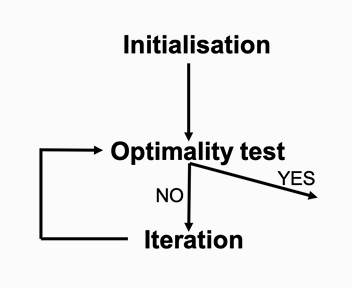
\includegraphics[width=0.3\textwidth]{graph1.png}
                \end{center} 
            
            \item \textbf{Come iniziare:}
            
                Quando possibile, l'inizializzazione del metodo del simplesso sceglie l'origine (tutte le variabili decisionali uguali a zero) come soluzione CPF iniziale. Quando ci sono troppe variabili decisionali per trovare graficamente una soluzione CPF iniziale, questa scelta elimina la necessità di utilizzare procedure algebriche per trovare e risolvere una soluzione CPF iniziale.
                
                La scelta dell'origine è comunemente possibile quando tutte le variabili decisionali hanno vincoli di non negatività, perché l'intersezione di questi confini dei vincoli produce l'origine come soluzione di punto d'angolo. Questa soluzione è quindi una soluzione CPF a meno che non sia infattibile perché viola uno o più vincoli. Se è infattibile, sono necessarie procedure speciali per trovare la soluzione CPF iniziale.
                

                \text{Oss: } non sempre è possibile scegliere l'origine come soluzione iniziale 
            
            \item \textbf{La scelta di una soluzione CPF migliore ad ogni iterazione}

                Data una soluzione CPF, è computazionalmente molto più veloce raccogliere informazioni sulle sue soluzioni CPF adiacenti rispetto ad altre soluzioni CPF. Pertanto, ogni volta che il metodo del simplesso esegue un'iterazione per passare dalla soluzione CPF corrente a una migliore, sceglie sempre una soluzione CPF che è adiacente a quella corrente. Non vengono considerate altre soluzioni CPF. Di conseguenza, l'intero percorso seguito per raggiungere infine una soluzione ottimale si snoda lungo i bordi della regione ammissibile.
            
            \item \textbf{Quale soluzione CPF adiacente scegliere ad ogni iterazione: }

                Dopo che la soluzione CPF corrente è stata identificata, il metodo del simplesso esamina ciascuno dei bordi della regione ammissibile che emanano da questa soluzione CPF e identifica il tasso di miglioramento in Z che si otterrebbe spostandosi lungo il bordo. Tra i bordi con un tasso di miglioramento positivo in Z, sceglie quindi di spostarsi lungo quello con il tasso di miglioramento maggiore in Z. L'iterazione è completata risolvendo prima per la soluzione CPF adiacente all'altra estremità di questo bordo e poi rietichettando questa soluzione CPF adiacente come la soluzione CPF corrente per il test di ottimalità e (se necessario) la successiva iterazione.
                
                Alla prima iterazione dell'esempio, spostarsi da (0, 0) lungo il bordo sull'asse $x_1$ darebbe un tasso di miglioramento in Z di 3 (Z aumenta di 3 per unità di aumento in $x_1$), mentre spostarsi lungo il bordo sull'asse $x_2$ darebbe un tasso di miglioramento in Z di 5 (Z aumenta di 5 per unità di aumento in $x_2$), quindi la decisione è di spostarsi lungo quest'ultimo bordo. Alla seconda iterazione, l'unico bordo che emana da (0, 6) che darebbe un tasso di miglioramento positivo in Z è il bordo che porta a (2, 6), quindi la decisione è di spostarsi successivamente lungo questo bordo.

            \item \textbf{Come viene eseguito efficacemente il test di ottimalità: }
            
                Un tasso di miglioramento positivo in Z implica che la soluzione CPF adiacente è migliore della soluzione CPF corrente, mentre un tasso di miglioramento negativo in Z implica che la soluzione CPF adiacente è peggiore. Pertanto, il test di ottimalità consiste semplicemente nel verificare se uno qualsiasi dei bordi dà un tasso di miglioramento positivo in Z. Se nessuno lo fa, allora la soluzione CPF corrente è ottima.
                
                Nell'esempio, spostarsi lungo entrambi i bordi da (2, 6) diminuisce Z. Poiché vogliamo massimizzare Z, questo fatto dà immediatamente la conclusione che (2, 6) è ottima.
            
        \end{itemize}

    \section{Soluzioni base}
        \subsection{Forma standard}
        Un qualuqnue problema di programmazione lineare può essere sempre formulato in FORMA STANDARD:
        \begin{align}
            \max{z} &= c^{T}x \notag \\
            Ax &= b, \text{ ($b \geq 0$)} \notag \\
            x & \geq 0 \notag 
        \end{align}

        \paragraph{Th. } per ogni PL $\exists$ PL' in forma standard

        \paragraph{}
        Dato il problema: 
        \begin{align}
            \max{z} &= cx \notag \\
                Ax &= b, \text{ } A \in M_{m,n}(\mathbb{R}) \notag \\
                x & \geq 0 \notag 
        \end{align}
        
        Si suppnga il $rango(A)$ = m, $m < n$, eventualmente riordinando le colonne, si può pore 
        \[
            A = [B|N]
        \]

        dove 
        \begin{itemize}
            \item B è una matrice nonsingolare $m \cdot n$ detta \textbf{matrice delle colonne base}
            \item N è una matrice $m \cdot (n-m)$, detta \textbf{matrice delle colonne fuori base}
        \end{itemize}

        La matrice B è composta da m colonne di A linearmente indipendenti che formano 
        una base nello spazio vettoriale ad m dimensioni delle colonne di A.



        \paragraph{}
        Sia:


        \[
            x = 
            \begin{pmatrix}
                x_1 \\
                \ldots \\
                x_n
            \end{pmatrix}
            \in \mathbb{R}^n
        \]

        In corripondenza di una scelta B e di N si può partizionare anche il vettore delle x:

        \[ x = 
        \begin{bmatrix}
            x_B \\
            x_N
        \end{bmatrix}
        \]

        \begin{itemize}
            \item $x_B$, costituito da $m$ componenti, è detto vettore delle variabili base (vettore base)
            \item $x_N$, costituito da $n-m$ componenti, è detto vettore delle variabili fuori base
        \end{itemize}



        \paragraph{}
        Il sistema di equazizoni lineari $Ax = b$ si può scrivere come:
        
        \begin{align}
            [B|N] 
            \begin{bmatrix}
                x_B \\
                x_N 
            \end{bmatrix} &= b
            \implies B x_B + N x_N = b \notag \\
            x_B &= B^{-1} b -B^{-1} N x_N \notag 
        \end{align}

        Dove $A = B|N$, B con $m$ elementi, invertibile, quindi $\exists$ $B^{-1}$, N di $(n-m)$ elementi.
        

        \paragraph{}
        Per ogni base B (matrice di base) ogni soluzione del sistema $Ax = b$ corrisponde a determinare il valore per $m$ variabuli $x_B$ avendo fissato arbitrariarmente il valore per le restanti $n-m$ varibiabili $x_N$.

        Una scelta particolarmente importante è porre $x_N = 0$, da cui si ottiene la corrispondente soluzione base: 
        
        \[ 
            x = 
            \begin{bmatrix}
                x_B \\
                x_N
            \end{bmatrix}
            = 
            \begin{bmatrix}
                B^{-1}b \\
                0
            \end{bmatrix}
        \]

        se $B^{-1} b \geq 0$ si ottiene una soluzione di base ammissibile (BFS) per il sistema $Ax = b$, $x \geq 0$


        \paragraph{}
        \textbf{Dato il problema $Ax = b,x \geq 0$, una soluzione x è un vertice del
        poliedro $P(A, b)$ se e solo se x è una BFS} (soluzione della base ammissibile)

        Un punto di un poliedro è un vertice (punto estremo) se e solo se soddisfa all’uguaglianza n vincoli linearmente indipendenti, quindi basta dimostrare che ogni BFS soddisfa n vincoli linearmente indipendenti tra $Ax = b,x \geq 0$.

        Per definizione ogni BFS soddisfa all’uguaglianza (n-m) vincoli $x \geq 0$ e gli m
        vincoli di $Ax = b$. I vincoli stringenti sono linearmente indipendenti poiché la matrice dei loro coefficienti è certamente non singolare essendo della forma
        

        \[
            \begin{pmatrix}
                B & N \\
                0 & I_{n-m}
            \end{pmatrix}
        \]

        \textbf{Problema LP-ESEMPIO: }

        \begin{align}
            \max_{x} z &= 2x_1+x_2 \notag \\
            x_1 + x_2 &\leq 5 \notag \\
            -x_1 + x+2 &\leq 0 \notag \\
            x_1 + 2x_2 &\leq 21 \notag \\
            x_1, x_2 &\geq 0 \notag 
        \end{align}

        Non è in forma standard, ma espresso solo in termini delle variabili strutturali (cioè che hanno un immediata corrispondenza
        fisica col sistema reale che viene modellato)

        \paragraph{OSS: } come lo si trasforma in \textbf{f. standard}? 

        Lo si trasforma in forma standard introducendo le variabili \textbf{SLACK} $s_1, s_2, s_3$. Sono variabili che rappresentano una sorta di "distanza" da uno dei vincoli. Se il valore è positivo siamo dentro al vincolo, se è 0 siamo sul vincolo, altrimenti siamo all'esterno del vincolo.

        \[
            \begin{cases}
                a+s = b \\
                s \geq 0
            \end{cases}
            \iff a \leq b 
        \]            
        
        Il problema ottenuto diventa quindi:

        \begin{align*}
            \max_{x} z &= 2x_1 + x_2 \\
            x_1 + x_2 + s_1 &= 5 \\
            -x_1 + x_2 + s_2 &= 0 \\
            6x_1 + 2x_2 + s_3 &= 21 \\
            x_1, x_2, s_1, s_2, s_3 &\geq 0.
        \end{align*}

        dove $s_1, s_2, s_3$ sono le variabili slack

        Se lo scriviamo nella forma matriciale ottengo:


        \begin{align*}
            \mathbf{A} &= 
            \begin{bmatrix}
            1 & 1 & 1 & 0 & 0 \\
            -1 & 1 & 0 & 1 & 0 \\
            6 & 2 & 0 & 0 & 1 \\
            \end{bmatrix},
            \mathbf{b} = 
                \begin{bmatrix}
                    5 \\
                    0 \\
                    21 \\
                \end{bmatrix}
        \end{align*}

        Limite superiore delle possibili basi $\frac{5!}{3!2!} = 10$, (alcune soluzioni sono degeneri, ovvero sono uguali; ex. 0 può essere ottenuto in più modi.), ma non tutte le basi corrispondono ad una soluzione ammissibile BFS, nell’esempio solo 6 basi sono ammissibili.

        Siccome i vertici sono 4, vi saranno BFS degeneri.      
        
        \paragraph{}
        \textbf{Esempio-BFS}

        \[
            \mathbf{x_B}^{(3)} =
            \begin{bmatrix}
                x_1 \\ x_2 \\s_2
            \end{bmatrix}
            \quad
            B_3 =
            \begin{bmatrix}
                1 & 1 & 0 \\
                -1 & 1 & 1 \\
                6 & 2 & 0
            \end{bmatrix}
            \quad
            B_3^{-1} =
            \frac{1}{4}
            \begin{bmatrix}
                -2 & 0 & 1 \\
                6 & 0 & -1 \\
                -8 & 4 & 2
            \end{bmatrix}
        \]
            
            

        \textbf{OSS: } come si capisce che un vertice è non ammissibile? Guardo alla soluzione se contiene dei valori $< 0$, in quel caso allora tale soluzione è non ammissibile.

        \paragraph{Oss: } $B_3$ è stato ricavato facendo (su gurobi) $A[x_B.index]$
        
        
        
        \[
            B_3^{-1} \mathbf{b} =
            B_3^{-1}
            \begin{bmatrix}
                5 \\ 0 \\ 21
            \end{bmatrix}
            =
            \begin{bmatrix}
                11/4 \\
                9/4 \\
                1/2
            \end{bmatrix}
            \Rightarrow p_3
        \]


        \[
            \mathbf{x}_B^{(2)} = \begin{bmatrix} x_1 \\ x_2 \\ s_3 \end{bmatrix} = \begin{bmatrix} 5/2 \\ 5/2 \\ 1 \end{bmatrix} \Rightarrow p_2
        \]


        \[
            \mathbf{x}_B^{(4)} = \begin{bmatrix} x_1 \\ s_1 \\ s_2 \end{bmatrix} = \begin{bmatrix} 7/2 \\ 3/2 \\ 7/2 \end{bmatrix} \Rightarrow p_4
        \]

        
        \[
            \mathbf{x}_B^{(1)} = \begin{bmatrix} x_1 \\ s_1 \\ s_3 \end{bmatrix} = \mathbf{x}_B^{(5)} = \begin{bmatrix} x_2 \\ s_1 \\ s_3 \end{bmatrix} = \mathbf{x}_B^{(6)} = \begin{bmatrix} s_2 \\ s_1 \\ s_3 \end{bmatrix} = \begin{bmatrix} 0 \\ 5 \\ 21 \end{bmatrix} \Rightarrow p_1
        \]


        \[
            \text{soluzioni degeneri}
        \]


        \[
            \mathbf{x_B}^{(7)} = \begin{bmatrix} x_1 \\ x_2 \\ s_1 \end{bmatrix} \quad \mathbf{B}_{(7)} = \begin{bmatrix} 1 & 1 & 1 \\ -1 & 1 & 0 \\ 6 & 2 & 0 \end{bmatrix} \quad \mathbf{B}_{(7)}^{-1} = \frac{1}{8} \begin{bmatrix} 0 & -2 & 1 \\ 0 & 6 & 1 \\ 8 & -4 & -2 \end{bmatrix}
        \]


        \[
            \mathbf{B}_{(7)}^{-1} \mathbf{b} = \mathbf{B}_{(7)}^{-1} \begin{bmatrix} 5 \\ 0 \\ 21 \end{bmatrix} = \begin{bmatrix} 21/8 \\ 21/8 \\ -1/4 \end{bmatrix}
        \]


        \[
            \text{Analogamente, sono basi non ammissibili}
        \]    


        \[
            \begin{bmatrix} x_2 \\ s_2 \\ s_3 \end{bmatrix} \quad \begin{bmatrix} x_1 \\ s_2 \\ s_3 \end{bmatrix} \quad \begin{bmatrix} x_2 \\ s_1 \\ s_2 \end{bmatrix}
        \]

        
        \subsubsection{Variabili surplus}
        Se in un problema di PL ci sono dei vincoli di maggiore o uguale, per trasformare il problema in forma standard si introducono delle variabili di surplus con segno opposto, ad esempio:

        \[
            -3x_1+2x_2 \geq 5 \Leftrightarrow -3x_1+2x_2 - s = 5 
        \]

        Esplicitando la funzione obiettivo:

        $$
            z = c\mathbf{x} = \begin{bmatrix} c_B & c_N \end{bmatrix} \begin{bmatrix} \mathbf{x}_B \\ \mathbf{x}_N \end{bmatrix} = c_B\mathbf{x}_B + c_N\mathbf{x}_N
        $$

        e sostituendo l'espressione delle variabili di base:

        $$
            \mathbf{x}_B = B^{-1}\mathbf{b} - B^{-1}N\mathbf{x}_N
        $$

        si ottiene:

        $$
            z = c_BB^{-1}\mathbf{b} - (c_BB^{-1}N - c_N)\mathbf{x}_N
        $$

        Il valore dell'obiettivo corrispondente alla base $B$ è quindi $z(B) = c_BB^{-1}\mathbf{b}$


            
    \section{Algoritmo del simplesso - fase I e fase II}
        Nell’algoritmo del simplesso si distingue una fase I, che consiste nel passo di inizializzazione in cui viene individuata una prima BFS, e una fase II, che consiste nel determinare la BFS ottima a partire dalla prima BFS.

        \paragraph{}
        La fase II è stata già illustrata, la fase I viene illustrata in seguito.

        \paragraph{}
        La verifica se il problema è illimitato può anche venire fatta durante la fase II controllando tutte le colonne associate a costi ridotti positivi (e quindi coefficienti nel tableau negativi), se le
        colonne sono numerose questa verifica può essere onerosa.

        In alcuni casi una prima base ammissibile è immediata. Si supponga infatti che il problema sia
        formulato come:

        \begin{align}
            \max{z} &= cx \notag \\
            Hx &\leq b \notag \\
            x &\geq 0 \notag 
        \end{align}

        con $b \geq 0$,allora la sua trasformazione in forma standard introduce delle variabili di slack s le cui corrispondenti colonne formano la prima base ammissibile: 

        \begin{align}
            \max{z} &= cx \notag \\
            Hx + Is & = b \notag \\
            x \geq 0, &s \leq 0 \notag 
        \end{align}

        Riordinando le colonne si ottiene: $A = [I | H], B = I$ e $N = H$

        dove chiaramente: $rango(A) = m$ e $B^{-1}b \le 0$

        \paragraph{}
        \textbf{def. }  Qualora un problema di PL in forma standard ha le matrice A che si può esprimere come

        $$
            A = [I | H] \text{, } \quad B = I \quad \text{ e }\quad N = H
        $$

        allora il problema è detto essere espresso in forma \textbf{canonica}

        \paragraph{}
        Non è immediato esprimere un problema di PL in forma canonica in presenza di disuguaglianze di verso opposto, infatti le variabili di \textbf{surplus} hanno coefficienti negativi, o in presenza di vincoli di uguaglianza.


        \paragraph{}
        \textbf{Esempio: }

        \begin{center}
            \begin{tabular}{ c | c }
                Formulazione iniziale & Formulazione standard \\
                
                $\min{z} = 4x_1 + x_2$ & $\max{z} = -4x_1 - x_2$ \\
                
                $3x_1 + x_2 = 3$ & $3x_1 + x_2 \quad \quad = 3$ \\
                
                $4x_1 + 3x_2 \geq 6$ & $4x_1 + 3x_2 - x_3 \quad \quad = 6$ \\
                
                $x_1 + 2x_2 \leq 4$ & $x_1 + 2x_2 \quad \quad + x_4 = 4$ \\
                
                $x_1, x_2 \geq 0$ & $x_1, x_2, x_3, x_4 \geq 0$ \\
            \end{tabular}
        \end{center}

        Questa formulazione standard NON è una forma canonica:
        
        \[
            A = 
            \begin{bmatrix}
                3 & 1 & 0 & 0 \\
                4 & 3 & -1 & 0 \\
                1 & 2 & 0 & 1 
            \end{bmatrix}
        \]

        Se il problema è nella forma standard, ottenuto solo da vincoli di tipo = e $\geq$, si introducono $m$ variabili artificiali $\mathbf{u}$ e si formula il problema di fase I

        $$
            \begin{array}{ccc}
                \max z = c\mathbf{x} & & \min w = \mathbf{1u} \\
                \mathbf{Ax} = \mathbf{b} & \Rightarrow \text{ fase I } & \mathbf{Ax} + \mathbf{Iu} = \mathbf{b} \\
                \mathbf{x} \geq 0 & & \mathbf{x} \geq 0, \mathbf{u} \geq 0
            \end{array}
        $$

        Per il problema di fase I è immediato determinare una base iniziale ammissibile.


        Il problema di fase I ammette una soluzione ottima $w^*$ non negativa per costruzione,

        \begin{itemize}
            \item se $w^* > 0$ allora il problema fase I non ha soluzioni ammissibili $\mathbf{x}$, $\mathbf{u}$ tali che $\mathbf{u} = 0$ e quindi non esiste $\mathbf{x}$ tale che $\mathbf{Ax} + \mathbf{I0} = \mathbf{b} \Rightarrow \mathbf{Ax} = \mathbf{b}$, da cui il sistema $\mathbf{Ax} = \mathbf{b}$ non è compatibile e il problema di PL non ha soluzioni ammissibili.
            \item se $w^* = 0$ allora la componente della soluzione ottima $\mathbf{x}^*$, $\mathbf{u}^*$ è tale che $\mathbf{u} = 0$ e quindi $\mathbf{x}^*$ è tale che $\mathbf{Ax}^* + \mathbf{I0} = \mathbf{b} \Rightarrow \mathbf{Ax}^* = \mathbf{b}$. Poiché $\mathbf{x}^*$ ha al più $m$ componenti non nulle, essa può essere presa come prima BFS del problema originale.
        \end{itemize}

        \paragraph{}
        \textbf{Esempio - Fase I}

        \begin{align*}
            \min w = u_1 + u_2 \quad  \Rightarrow \max w = -u_1 - u_2 \\
            3x_1 + x_2 \quad \quad  + u_1 \quad  = 3 \\
            4x_1 + 3x_2 - x_3 \quad \quad + u_2 = 6 \\
            x_1 + 2x_2  \quad + x_4 \quad \quad  = 4 \\
            x_1, x_2, x_3, x_4, u_1, u_2 \geq 0
        \end{align*}
            
        Data la presenza di una variabile di slack, sono necessarie solo due variabili artificiali ($u_1$, $u_2$).

        \paragraph{}
        $u_1, u_2, x_4$ è la base iniziale.

        \paragraph{}
        \textbf{Esempio: radioterapia}

    \section{Il problema duale}
        
        \subsection{A production problem}
        Un'azienda produce $n$ beni diversi utilizzando $m$ materie prime diverse.

        \begin{itemize}
            \item Sia $b_i$, per $i = 1, \dots, m$, la quantità disponibile della $i$-esima materia prima.
            \item Il $j$-esimo bene, per $j = 1, \dots, n$, richiede $a_{ij}$ unità della $i$-esima materia prima e genera un ricavo $c_j$ per unità prodotta.
        \end{itemize}

        L'azienda si trova di fronte al problema di decidere quanto produrre di ciascun bene al fine di massimizzare i suoi ricavi totali.

        La variabile di decisione è definita come segue:

        Sia $x_j$, per $j = 1, \dots, n$, la quantità del $j$-esimo bene da produrre.


        \subsection{Primal Formulation}

        \begin{align*}
            \max{z} =  c_{1}x_{1} + \dots + c_{n}x_{n} \\
            \quad a_{i1}x_{1} + \dots + a_{in}x_{n} \leq b_{i}, \quad i=1, \dots, m \\
            \quad x_{j} \geq 0, \quad j=1, \dots, n
        \end{align*}

        \paragraph{Variabili di decisione:} la quantità di beni prodotti:
        \[ x_j \in \mathbb{R}, \quad \forall j=1,\dots,n. \]
        Queste variabili sono considerate continue.

        \paragraph{Funzione obiettivo:} massimizzare il profitto:
        \[ \sum_{j=1}^{n} c_j x_j. \]

        \paragraph{Vincoli:} per ciascuna materia prima, la quantità utilizzata nella produzione non può superare la quantità disponibile:
        \[ \sum_{j=1}^{n} a_{ij} x_j \leq b_i, \quad \forall i=1,\dots,m. \]
        Per ciascun bene, la quantità di produzione deve essere non negativa:
        \[ x_j \geq 0, \quad \forall j=1,\dots,n. \]

        \paragraph{Esempio: }

        \begin{align*}
            \max & \quad 15x_{1} + 10x_{2} \\
            (R_p)& \quad x_{1} + x_{2} \leq 2000 \\
            (R_q) & \quad x_{1} + 0.5x_{2} \leq 1000 \\
            (R_r) & \quad 2x_{1} + x_{2} \leq 3000 \\
            & \quad x_{1}, x_{2} \geq 0
        \end{align*}

        \paragraph{Commenti sul problema primale}
        Prima di decidere la produzione per massimizzare il profitto, si dovrebbe considerare se è più vantaggioso vendere le materie prime invece di produrre beni.

        La domanda chiave è:

        \textit{Qual è il prezzo minimo al quale tutte le risorse disponibili dovrebbero essere vendute piuttosto che utilizzate per la produzione?}

        La risposta a questa domanda è data dal \textbf{problema duale}.

        \paragraph{}
        \textbf{Il duale del problema di produzione}
        Assumendo la linearità, il profitto totale dalla vendita delle risorse è uguale alla somma dei profitti ottenuti dalla vendita di ciascuna risorsa individuale. Il profitto dalla vendita di un'unità di un bene non deve superare il profitto ottenuto dalla vendita delle materie prime necessarie.
        
        \paragraph{}
        Un bene $P_1$ dà un profitto di 15 e consuma un'unità di $R_p$, un'unità di $R_q$ e 2 unità di $R_r$. Pertanto, per rendere conveniente vendere le risorse (o almeno rimanere alla pari) invece di produrre, la vendita complessiva di un'unità di $R_p$, un'unità di $R_q$ e 2 unità di $R_r$ deve fornire un guadagno non inferiore a 15.

        I prezzi di vendita delle risorse devono essere non negativi.

        \subsection*{Variabili duali e Funzione obiettivo}

            
            \textbf{Variabili decisionali}
            Prezzo unitario di ciascuna risorsa:
            \[ \pi_i \in \mathbb{R}, \quad \forall i = 1, \dots, m. \]
            Queste sono variabili continue.

        \subsection*{Funzione obiettivo}
            Massimizzare il profitto dalla vendita delle risorse:
            \[ 
                \sum_{i=1}^{m} b_i \pi_i = 
            \]

            \[
                = 2000 \pi_p + 1000 \pi_q + 3000 \pi_r
            \]

        \subsection*{Vincoli duali}
            Per ciascun bene, il costo delle materie prime deve essere almeno pari al profitto derivante dalla produzione del bene:
            \[ \sum_{i=1}^{m} a_{ij} \pi_i \geq c_j, \quad \forall j=1,2 \]
            I prezzi delle risorse devono essere non negativi:
            \[ \pi_i \geq 0, \quad \forall i=p,q,r \]

        \subsection*{Formulazione duale}

            \begin{align*}
                \textcolor{green}{\text{(profit)}} \quad \quad &\min q = 2000\pi_p + 1000\pi_q + 3000\pi_r \\
                \textcolor{green}{\text{(product 1)}} \quad & \pi_p + \pi_q + 2\pi_r \geq 15 \\
                \textcolor{green}{\text{(product 2)}} \quad & \pi_p + 0.5\pi_q + \pi_r \geq 10 \\
                & \pi_p, \pi_q, \pi_r \geq 0
            \end{align*}
            
            \begin{align*}
                \min \sum_{i=1}^{m} b_i \pi_i & \\
                \sum_{i=1}^{m} a_{ij} \pi_i \geq c_j \qquad & \text{for } j = 1, \dots, n \\
                \pi_i \geq 0 \qquad & \text{for } i = 1, \dots, m
            \end{align*}
                
            in forma matriciale:
            \begin{align*}
                \min b^T \pi \\
                A^T \pi \geq c
                \quad \pi \geq 0
            \end{align*}

        \subsection*{Commenti sul problema duale}

            È intuitivamente evidente che:

            \begin{itemize}
                \item Qualsiasi soluzione ammissibile al problema duale garantisce un profitto non inferiore al massimo ottenibile attraverso la produzione.
                \item La soluzione duale ottima non può essere inferiore alla soluzione primale ottima, altrimenti la produzione sarebbe ancora vantaggiosa.
            \end{itemize}

        \subsection{Problema primale e duale}            
                        
            \noindent Ad ogni problema di programmazione lineare (primale) è associato un problema duale

            \paragraph{}
            \noindent\begin{minipage}{0.48\textwidth}
            \noindent \textcolor{orange}{\textbf{Problema primale (P)}}

            \noindent \begin{align*}
            \max z = c_1 x_1 +& \dots + c_n x_n \\
            a_{11} x_1 +& \dots + a_{1n} x_n \leq b_1 \\
            & \vdots \\
            a_{m1} x_1 +& \dots + a_{mn} x_n \leq b_m \\
            x_1, \dots, x_n &\geq 0
            \end{align*}

            \noindent \textit{n variabili e m vincoli}
            \end{minipage}
            \hfill
            \begin{minipage}{0.48\textwidth}
            \noindent \textcolor{cyan}{\textbf{Problema duale (D)}}

            \noindent \begin{align*}
            \min w = b_1 \pi_1 +& \dots + b_m \pi_m \\
            a_{11} \pi_1 +& \dots + a_{m1} \pi_m \geq c_1 \\
            & \vdots \\
            a_{1n} \pi_1 +& \dots + a_{mn} \pi_m \geq c_n \\
            \pi_1, \dots, \pi_m &\geq 0
            \end{align*}

            \noindent \textit{m variabili e n vincoli}
            \end{minipage}

            \paragraph{}
            \textbf{Proprietà: } il problema D ha tante variabili quanti sono i vincoli in P e tanti vincoli quante sono le variabili in P.

            \paragraph{}
            \noindent In forma matriciale, vediamo che i vettori $b$ e $c$ scambiano le loro posizioni e la matrice dei coefficienti $A$ è trasposta.

            \paragraph{}
            \noindent\begin{minipage}{0.48\textwidth}
            \noindent \textcolor{orange}{\textbf{Problema primale (P)}}

            \noindent \begin{align*}
            \max z &= c^T x \\
            Ax &\leq b \\
            x &\geq 0 \\
            x &\in \mathbb{R}^n
            \end{align*}
            \end{minipage}
            \hfill
            \begin{minipage}{0.48\textwidth}
            \noindent \textcolor{cyan}{\textbf{Problema duale (D)}}

            \noindent \begin{align*}
            \min w &= b^T \pi \\
            A^T \pi &\geq c \\
            \pi &\geq 0 \\
            \pi &\in \mathbb{R}^m
            \end{align*}
            \end{minipage}
        \subsection*{Osservazioni: }

        La dualità non sorge solo da giustificazioni economiche, ma anche dall'applicazione delle condizioni di Kuhn-Tucker ai problemi di programmazione lineare o dal rilassamento Lagrangiano.

        La dualità è importante perché:

        \begin{itemize}
            \item il problema duale corrisponde a una diversa visione dello stesso problema (per il quale deve sempre essere ricercata un'interpretazione economica della formulazione ottenuta);
            \item su di essa si basano algoritmi, come il Dual Simplex e l'Algoritmo Primale-Duale, alternativi al Simplex (Primale), che sono utili per certe classi di problemi;
            \item in alcuni casi può essere conveniente risolvere D invece di P (potrebbe essere meglio risolvere il problema con meno vincoli).
        \end{itemize}

    \subsection{Primal-Dual Relationship}
        \begin{table}[h!]
            \centering
            \begin{tabular}{|c|c||c|c|}
            \hline
            PRIMALE & massimizzare & minimizzare & DUALE \\
            \hline
            vincoli & $\leq b_i$ & $\geq 0$ & variabili \\
             & $\geq b_i$ & $\leq 0$ & \\
             & $= b_i$ & libere & \\
            \hline
            variabili & $\geq 0$ & $\geq c_j$ & vincoli \\
             & $\leq 0$ & $\leq c_j$ & \\
             & libere & $=$ & \\
            \hline
            \end{tabular}
        \end{table}

        \paragraph{}
        \textbf{Esempi}
        Problema primale (P)
        \begin{align*}
            \max z &= 2x_1 + 3x_2 - x_3 + 7x_4 \\
            4x_1 + 3x_2 - x_3 + 2x_4 &\leq 35 \quad (\pi_1) \\
            x_1 + 5x_2 + 6x_3 + 10x_4 &= 28 \quad (\pi_2) \\
            2x_1 + 7x_2 - 2x_3 + 4x_4 &\geq 15 \quad (\pi_3) \\
            x_1 \geq 0, x_2 \text{ libera }, x_3 \leq 0, x_4 &\geq 0
        \end{align*}
        
        Problema duale (D)
        \begin{align*}
            \min w &= 35\pi_1 + 28\pi_2 + 15\pi_3 \\
            4\pi_1 + \pi_2 + 2\pi_3 &\geq 2 \quad (x_1) \\
            3\pi_1 + 5\pi_2 + 7\pi_3 &= 3 \quad (x_2) \\
            -\pi_1 + 6\pi_2 - 2\pi_3 &\leq -1 \quad (x_3) \\
            2\pi_1 + 10\pi_2 + 4\pi_3 &\geq 7 \quad (x_4) \\
            \pi_1 \geq 0, \pi_2 \text{ libera }, \pi_3 &\leq 0
        \end{align*}
        
        \subsection{Risultati importanti: }
        \textbf{Th. della dualità (debole):} se $x$ è una soluzione ammissibile per il problema primale e $\pi$ è una soluzione ammissibile per il problema duale allora
        
        \begin{equation*}
            c^T x \leq b^T \pi
        \end{equation*}
        
        \textbf{Dim. } Infatti,

        \begin{equation*}
            c^T x \leq (A^T \pi)^T x = \pi^T A x \leq \pi^T b = b^T \pi
        \end{equation*}
    
        \textbf{Corollari: }
        \begin{enumerate}
            \item Se il valore ottimo nel primale è $+\infty$, allora il problema duale deve essere inammissibile
            \item Se il valore ottimo nel duale è $-\infty$, allora il problema primale deve essere inammissibile
        \end{enumerate}

        \textbf{Dim.} Supponiamo che il valore ottimo nel problema primale sia $+\infty$ e che il problema duale abbia una soluzione ammissibile $\pi$. Per dualità debole, $\pi$ soddisfa $b^T \pi \geq c^T x$ per ogni primale ammissibile $x$. Prendendo il massimo su tutti gli $x$ ammissibili, concludiamo $b^T \pi \geq +\infty$. Questo è impossibile e mostra che il duale non può avere una soluzione ammissibile, stabilendo così la parte (a). La parte (b) segue da un argomento simmetrico.
        
        \paragraph{}
        \textbf{Corollario: } siano $x$ e $\pi$ soluzioni ammissibili per il primale e il duale, rispettivamente, e supponiamo che $c^T x = b^T \pi$. Allora $x$ e $\pi$ sono soluzioni ottime per il primale e il duale, rispettivamente.

        \paragraph{}
        \textbf{Dim.} Siano $x$ e $\pi$ come nell'enunciato del corollario. Per ogni soluzione ammissibile primale $y$, il teorema della dualità debole produce $c^T x = b^T \pi \geq c^T y$, il che dimostra che $x$ è ottimo. La dimostrazione dell'ottimalità di $\pi$ è simile.
        
        \paragraph{}
        \textbf{Th. dualità forte:} se un problema di programmazione lineare ha una soluzione ottima, allora anche il suo duale ce l'ha, e i rispettivi valori ottimi sono uguali.
        
        \paragraph{}
        In altre parole, se $x^*$ è una soluzione ottima finita per il primale, anche il duale ha una soluzione ottima finita $\pi^*$ ed è sempre vero che $c^T x^* = b^T \pi^*$.
        
        \subsubsection*{Relazioni tra Primale e Duale}
        Ricordiamo che in un problema di programmazione lineare, si verificherà esattamente una delle seguenti tre possibilità
        \begin{enumerate}
            \item Esiste una soluzione ottima
            \item Il problema è "illimitato", cioè il valore ottimo è $+\infty$ (per i problemi di massimizzazione) o $-\infty$ (per i problemi di minimizzazione)
            \item Il problema è inammissibile
        \end{enumerate}

        Questo porta a nove possibili combinazioni per il primale e il duale:

        \begin{table}[ht]
            \centering
            \begin{tabular}{c|c|c|c}
                & Ottimo finito & Illimitato & Inammissibile \\
                Ottimo finito & Possibile & Impossibile & Impossibile \\
                Illimitato & Impossibile & Impossibile & Possibile \\
                Inammissibile & Impossibile & Possibile & Possibile \\
            \end{tabular}
        \end{table}
        \paragraph{}
        \textbf{Esempio: due problemi inammissibili (si D che P)}
        Considera il primale inammissibile
        \begin{align*}
            \min x_1 + 2x_2 \\
            x_1 + x_2 = 1 \\
            2x_1 + 2x_2 = 3 \\
            x_1, x_2 \text{ libera }
        \end{align*}
        Il suo duale è
        \begin{align*}
            \max \pi_1 + 3\pi_2 \\
            \pi_1 + 2\pi_2 = 1 \\
            \pi_1 + 2\pi_2 = 2 \\
            \pi_1, \pi_2 \text{ libera }
        \end{align*}
        che è anche inammissibile.
        
        \paragraph{}
        \textbf{Complementarietà: } siano $x$ e $\pi$ soluzioni ammissibili per il problema primale e il problema duale, rispettivamente. I vettori $x$ e $\pi$ sono soluzioni ottime per i due rispettivi problemi se e solo se

        \begin{align*}
            \pi_i(b_i - a^T_i x) &= 0 \quad \forall i \\
            (\pi^T A_j - c_j)x_j &= 0 \quad \forall j,
        \end{align*}
        dove $A_j$ è la $j$-esima colonna e $a_i$ è la $i$-esima riga della matrice A.
        
        \paragraph{}
        \textbf{Dim. }
        \textbf{se (x, $\pi$) sono ottimi: } I vincoli dei problemi impongono che $\pi^T b \geq \pi^T A x \geq c^T x$.
        Poiché $x$ e $\pi$ sono ottimi $\pi^T b = c^T x$, quindi $\pi^T b = \pi^T A x$ e pertanto
        $\pi(b^T - Ax) = 0$. Allo stesso modo, ne consegue che $(\pi^T A - c^T)x = 0$. Infine, poiché $\pi \geq 0$,
        $b^T - Ax \geq 0$, $\pi^T A - c^T \geq 0$, $x \geq 0$, ne consegue che ogni termine dei prodotti scalari deve essere uguale a zero, cioè, $\pi_i(a^T_i x - b_i) = 0 \quad \forall i$ e
        $(c_j - \pi^T A_j)x_j = 0 \quad \forall j$.
        \newline
        \textbf{se le equazioni valgono:  } Scrivendo le equazioni in forma compatta e per la coppia
        (x, $\pi$) tale che
        \begin{align*}
            \pi(b^T - Ax) = 0 \Rightarrow \pi b^T = \pi Ax
        \end{align*}
        e
        \begin{align*}
            (\pi^T A - c^T)x = 0 \Rightarrow \pi Ax = c^T x
        \end{align*}
        poiché $\pi^T b = \pi^T Ax = c^T x$, allora (x, $\pi$) è ottimo.
        
        \paragraph{}
        \textbf{Osservazioni sulla complementarità}

        \begin{itemize}
            \item il teorema della complementarità può essere riformulato affermando che se un vincolo primale non è stretto (cioè, è $<$) allora la variabile duale associata deve essere nulla, viceversa se una variabile duale è non nulla il vincolo primale associato deve essere stretto (cioè, $=$).
            \item può accadere che il vincolo sia stretto e la variabile duale associata sia nulla.
        \end{itemize}
        
        \paragraph{}
        \textbf{Esercizi:} scrivere il duale dei seguenti problemi 
        
        \begin{alignat*}{3}
            &\textbf{Es. 1} &\qquad\qquad &\textbf{Es. 2} \\
            &\max 5x_1 + 2x_2 + 3x_3 &\qquad\qquad &\max 0 \\
            &x_1 - 2x_2 + 5x_3 = 4 &\qquad\qquad &3x_1 - 2x_2 + 8x_3 \leq 4 \\
            &2x_1 + 7x_2 + 2x_3 \geq 10 &\qquad\qquad &7x_1 + 7x_2 + 9x_3 \leq 10 \\
            &2x_1 + 4x_3 \leq 5 &\qquad\qquad &x_1 + 10x_3 \leq 5 \\
            &x_1, x_2, x_3 \geq 0 &\qquad\qquad &x_1, x_2, x_3 \text{ libera }
        \end{alignat*}
        
        \section*{Soluzioni}
        
        \begin{alignat*}{3}
            &\textbf{Es. 1} &\qquad\qquad &\textbf{Es. 2} \\
            &\min 4\pi_1 + 10\pi_2 + 5\pi_3 &\qquad\qquad &\min 4\pi_1 + 10\pi_2 + 5\pi_3\\
            &\pi_1 + 2\pi_2 + 2\pi_3 \geq 5 &\qquad\qquad &3\pi_1 + 7\pi_2 + \pi_3 = 0\\
            &-2\pi_1 + 7\pi_2 \geq 2 &\qquad\qquad &-2\pi_1 + 7\pi_2 = 0 \\
            &5\pi_1 + 2\pi_2 + 4\pi_3 \geq 3 &\qquad\qquad &8\pi_1 + 9\pi_2 + 10\pi_3 = 0\\
            &\pi_1 \text{ libera }, \pi_2 \leq 0, \pi_3 \geq 0 &\qquad\qquad &\pi_1, \pi_2, \pi_3 \geq 0
        \end{alignat*}


    \section{Dualità e analisi di sensitività}

        \subsection{Un problema rilassato}
        Considera il problema in forma standard

        \begin{align*}
            &\min c^T x \\
            & Ax = b \\
            & x \geq 0
        \end{align*}

        che chiamiamo il problema \textbf{primale}, e sia $x^*$ una soluzione ottima, supposta esistere. Introduciamo un problema \textbf{rilassato} in cui il vincolo $Ax = b$ è sostituito da una penalità $p^T (b - Ax)$, dove $p$ è un vettore della stessa dimensione di $b$. Ci troviamo quindi di fronte al problema

        
        \begin{align*}
            & \min c^T x + p^T (b - Ax) \\
            & x \geq 0.
        \end{align*}
        

        Sia $g(p)$ il costo ottimale per il problema rilassato, in funzione del vettore $p$. Il problema rilassato consente più opzioni di quelle presenti nel problema primale, e ci aspettiamo che $g(p)$ non sia maggiore del costo ottimale $c^T x^*$. Infatti,

        \[
            g(p) = \min_{x \geq 0} [c^T x + p^T (b - Ax)] \leq c^T x^* + p^T (b - Ax^*) = c^T x^*
        \]

        dove l'ultima uguaglianza segue dal fatto che $x^*$ è una soluzione ammissibile per il problema primale, e soddisfa $Ax^* = b$. Quindi, ogni $p$ porta a un limite inferiore $g(p)$ per il costo ottimale $c^T x^*$.



        \subsection{Uno stretto Bound}
        Il problema

        \[
        \begin{aligned}
            &\max g(p) \\
            & \text{nessun vincolo}
        \end{aligned}
        \]

        può essere interpretato come una ricerca del limite inferiore più stretto possibile di questo tipo, ed è noto come il problema \textbf{duale}.

        \subsection{Il problema duale}
        Usando la definizione di $g(p)$, abbiamo

        \[
        g(p) = \min_{x \geq 0} [c^T x + p^T (b - Ax)] = p^T b + \min_{x \geq 0} (c^T - p^T A)x
        \]

        Nota che

        \[
        \min_{x \geq 0} (c^T - p^T A)x = \begin{cases}
        0 & \text{se } c^T - p^T A \geq 0 \\
        -\infty & \text{altrimenti (x -> +inf)}
        \end{cases}
        \]

        Nel massimizzare $g(p)$ dobbiamo considerare solo quei valori di $p$ per cui $g(p)$ non è uguale a $-\infty$. Concludiamo quindi che il problema duale è lo stesso di

        \[
        \begin{aligned}
            & \max p^T b \\
            & p^T A \leq c^T
        \end{aligned}
        \]

        (se cerchiamo il max $g(p)$ allora $c^T - p^T A \geq 0$)

        \paragraph{}
        Nell'esempio, abbiamo iniziato con vincoli di uguaglianza $Ax = b$ e abbiamo finito senza vincoli sul segno del vettore $p$. Se il problema primale avesse invece vincoli di disuguaglianza della forma $Ax \geq b$, potrebbero essere sostituiti da $Ax - s = b$, $s \geq 0$. I vincoli di uguaglianza possono essere scritti nella forma

        \[
            [A | -I] \begin{bmatrix} x \\ s \end{bmatrix} = b,
        \]

        il che porta ai vincoli duali

        \[
            p^T [a | -I] \leq [c^T | 0^T],
        \]

        o equivalentemente,

        \[
            p^T A \leq c^T, p \geq 0.
        \]

        Se il vettore $x$ è libero piuttosto che vincolato nel segno, usiamo il fatto

        \[
        \min_{x} (c^T - p^T A)x = 
        \begin{cases}
            0 & \text{se } c^T - p^T A = 0 \\
            -\infty & \text{altrimenti}
        \end{cases}
        \]

        per finire con i vincoli $p^T A = c^T$ nel problema duale. Queste considerazioni motivano le relazioni primale-duale.

        \begin{table}[h!]
            \centering
            \begin{tabular}{|c|c||c|c|}
            \hline
            PRIMALE & massimizzare & minimizzare & DUALE \\
            \hline
            vincoli & $\leq b_i$ & $\geq 0$ & variabili \\
             & $\geq b_i$ & $\leq 0$ & \\
             & $= b_i$ & libere & \\
            \hline
            variabili & $\geq 0$ & $\geq c_j$ & vincoli \\
             & $\leq 0$ & $\leq c_j$ & \\
             & libere & $=$ & \\
            \hline
            \end{tabular}
        \end{table}



        \subsection{L'analisi di sensitività}

        Lo scopo principale dell'analisi di sensitività è identificare i parametri sensibili (cioè, quelli che non possono essere cambiati senza cambiare la soluzione ottima). I parametri sensibili sono i parametri che devono essere stimati con particolare attenzione per minimizzare il rischio di ottenere una soluzione ottima errata.

        I parametri del modello in esame sono gli $a_{ij}$, $b_i$, $c_j$ per $i = 1, \dots, m$ e $j = 1, \dots, n$.

        
        





































        

        \begin{itemize}
            \item I problemi di programmazione lineare spesso possono essere interpretati come allocazione di risorse alle attività.
            \item Quando i vincoli sono nella forma $\leq$, interpretiamo i $b_i$ (i lati destri) come le quantità delle rispettive risorse rese disponibili per le attività in esame.
            \item In molti casi, i valori $b_i$ utilizzati nel modello iniziale possono effettivamente rappresentare la decisione iniziale provvisoria della direzione su quanta parte delle risorse dell'organizzazione sarà fornita alle attività considerate nel modello.
            \item Da questa prospettiva più ampia, alcuni dei valori $b_i$ possono essere aumentati in un modello rivisto, ma solo se si può presentare alla direzione un caso sufficientemente forte che questa revisione sarebbe vantaggiosa.
        \end{itemize}




        \textbf{prezzo ombra}

        \textbf{Definizione}

        Il \textit{prezzo ombra} per la risorsa $i$ (denotato da $y_i^*$) misura il valore marginale di questa risorsa, cioè, il tasso al quale $Z$ potrebbe essere aumentato aumentando (di poco) la quantità di questa risorsa ($b_i$) resa disponibile.





        Il grafico mostra che il prezzo ombra è $y_2^* = \frac{3}{2}$ per la risorsa 2. I due punti sono le soluzioni ottimali per $b_2 = 12$ o $b_2 = 13$, e inserendo queste soluzioni nella funzione obiettivo si rivela che aumentare $b_2$ di 1 aumenta $Z$ di $\frac{3}{2}$.

        Dimostra che $y_2^* = \frac{3}{2}$ è il tasso al quale $Z$ potrebbe essere aumentato aumentando $b_2$ "leggermente". Tuttavia, dimostra anche il fenomeno comune che questa interpretazione vale solo per un piccolo aumento di $b_2$. Una volta che $b_2$ viene aumentato oltre 18, la soluzione ottima rimane a $(0, 9)$ senza ulteriori aumenti di $Z$.

        In altre parole, $Z = 45$ per qualsiasi $b_2$ tale che $b_2 \geq 18$ perché il vincolo $2x_2 = b_2$ diventa ridondante.



        Nota che $y_1^* = 0$. Poiché il vincolo sulla risorsa 1, $x_1 \leq 4$, non è vincolante sulla soluzione ottima $(2, 6)$, c'è un surplus di questa risorsa. Pertanto, aumentare $b_1$ oltre 4 non può produrre una nuova soluzione ottima con un valore maggiore di $Z$.

        Al contrario, i vincoli sulle risorse 2 e 3, $2x_2 \leq 12$ e $3x_1 + 2x_2 \leq 18$, sono \textit{vincoli vincolanti} (vincoli che valgono con l'uguaglianza alla soluzione ottima). Poiché la fornitura limitata di queste risorse ($b_2 = 12$, $b_3 = 18$) impedisce a $Z$ di essere ulteriormente aumentato, hanno prezzi ombra positivi. Possiamo facilmente dimostrare che $y_3^* = 1$.

        Gli economisti si riferiscono a tali risorse come \textit{beni scarsi}, mentre le risorse disponibili in surplus (come la risorsa 1) sono \textit{beni liberi} (risorse con un prezzo ombra zero).



        Nota che $y_1^* = 0$. Poiché il vincolo sulla risorsa 1, $x_1 \leq 4$, non è vincolante sulla soluzione ottima $(2, 6)$, c'è un surplus di questa risorsa. Pertanto, aumentare $b_1$ oltre 4 non può produrre una nuova soluzione ottima con un valore maggiore di $Z$.

        Al contrario, i vincoli sulle risorse 2 e 3, $2x_2 \leq 12$ e $3x_1 + 2x_2 \leq 18$, sono \textit{vincoli vincolanti} (vincoli che valgono con l'uguaglianza alla soluzione ottima). Poiché la fornitura limitata di queste risorse ($b_2 = 12$, $b_3 = 18$) impedisce a $Z$ di essere ulteriormente aumentato, hanno prezzi ombra positivi. Possiamo facilmente dimostrare che $y_3^* = 1$.

        Gli economisti si riferiscono a tali risorse come \textit{beni scarsi}, mentre le risorse disponibili in surplus (come la risorsa 1) sono \textit{beni liberi} (risorse con un prezzo ombra zero).



        Le condizioni di complementarità sono

        \[
        \begin{aligned}
        \pi_i (b_i - a_i^T x^*) &= 0 \quad \forall i \\
        (\pi^T A_j - c_j)x_j^* &= 0 \quad \forall j,
        \end{aligned}
        \]

        che nel nostro caso diventano

        \[
        \begin{aligned}
        \pi_1 (4 - x_1^*) &= 0 \\
        \pi_2 (12 - 2x_2^*) &= 0 \\
        \pi_3 (18 - 3x_1^* - 2x_2^*) &= 0 \\
        (\pi_1^* + 3\pi_3 - 3) x_1^* &= 0 \\
        (2\pi_2^* + 2\pi_3 - 5) x_2^* &= 0
        \end{aligned}
        \]

        Poiché $x_1^* = 2$, $x_2^* = 6$ allora

        \[
        \begin{aligned}
        2 \times \pi_1^* &= 0 \\
        0 \times \pi_2^* &= 0 \\
        0 \times \pi_3^* &= 0 \\
        2 \times (\pi_1^* + 3\pi_3 - 3) &= 0 \\
        6 \times (2\pi_2^* + 2\pi_3 - 5) &= 0
        \end{aligned}
        \]


        Ne consegue che

        \[
        \begin{aligned}
        \pi_1^* &= 0 \\
        (\pi_1^* + 3\pi_3^* - 3) &= 0 \\
        (2\pi_2^* + 2\pi_3^* - 5) &= 0
        \end{aligned}
        \]

        Cioè

        \[
        \begin{aligned}
        \pi_1^* &= 0 \\
        \pi_3^* &= 1 \\
        \pi_2^* &= \frac{3}{2}
        \end{aligned}
        \]

        Infatti, $w^* = 4 \times 0 + 12 \times \frac{3}{2} + 18 \times 1 = 36$. Inoltre, notiamo che

        \[
        y_i^* = \pi_i^* \quad \text{per} \quad i = 1, 2, 3.
        \]

        Le variabili duali ottimali sono (uguali a) i prezzi ombra.





        Abbiamo dimostrato che ogni variabile duale ottima rappresenta il tasso al quale $Z$ varia variando il corrispondente valore del lato destro.

        Se variamo un lato destro, il valore delle variabili duali ottimali rimane costante fintanto che la soluzione ottima si trova sull'intersezione degli stessi confini dei vincoli.

        Nel nostro esempio,

        \begin{itemize}
            \item se $b_2 > 18$ la soluzione ottima è sempre $(0, 9)$. Le variabili duali ottimali sono $(0, 0, 5/2)$
            \item se $b_2$ varia nell'intervallo $6 < b_2 < 18$ la soluzione ottima si trova sull'intersezione tra $2x_2 = b_2$ e $3x_1 + 2x_2 = 18$ e le variabili duali ottimali sono $(0, 3/2, 1)$.
            \item se $0 < b_2 < 6$ la soluzione ottima si trova sull'intersezione tra $2x_2 = b_2$ e $x_1 = 4$. Le variabili duali ottimali sono $(3, 5/2, 0)$.
            \item se $b_2 = 6$ o $b_2 = 18$ la soluzione è chiamata \textbf{degenere}.
        \end{itemize}


        Il grafico dimostra l'analisi di sensitività di $c_1$ e $c_2$ per il nostro problema. A partire dalla linea della funzione obiettivo originale [dove $c_1 = 3$, $c_2 = 5$, e la soluzione ottima è $(2, 6)$], le altre due linee nere mostrano gli estremi di quanto può cambiare la pendenza della linea della funzione obiettivo e conservare comunque $(2, 6)$ come soluzione ottima. Pertanto,

        \begin{itemize}
            \item con $c_2 = 5$, l'intervallo ammissibile per $c_1$ è $0 \leq c_1 \leq 7.5$,
            \item con $c_1 = 3$, l'intervallo ammissibile per $c_2$ è $c_2 \geq 2$.
        \end{itemize}



        \section*{Come risolvere un IP?}

        Enumerazione. Tutte le soluzioni ammissibili sono identificate e la migliore è selezionata. Potrebbe non essere praticamente fattibile. Ad esempio, per risolvere il TSP in un grafo completo con n nodi ci sono $(n-1)!$ tour ammissibili. Quindi,

        Sono necessarie idee migliori.

        \begin{center}
        \begin{tabular}{cc}
        n & n! \\
        10 & $3.6\times10^{6}$ \\
        100 & $9.33\times10^{157}$ \\
        1000 & $4.02\times10^{2567}$
        \end{tabular}
        \end{center}

        \section*{Il problema del commesso viaggiatore}

        Ci viene dato un insieme di nodi $V=\{1,...,n\}$ (ad esempio, città) e un insieme di archi A.

        Gli archi rappresentano coppie ordinate di città tra le quali è possibile il viaggio diretto.

        Per $(i,j)\in\mathcal{A}$, $c_{ij}$ è il tempo di viaggio diretto dalla città i alla città j.
        Il TSP mira a trovare un tour, a partire dalla città 1, che

        a) visita ogni altra città esattamente una volta e poi ritorna alla città 1
        b) richiede il minor tempo di viaggio totale

        Il problema del commesso viaggiatore (TSP)

        Un tour che visita tutti i nodi esattamente una volta è chiamato tour Hamiltoniano.
        Il TSP identifica il tour Hamiltoniano di costo minimo.

        \section*{TSP - sembra facile}


        Tre tour: A-B-D-C-A: 11; A-D-B-C-A: 23; A-D-C-A: 18.

        \section*{TSP - forse non troppo facile}


        \section*{TSP - è difficile!!}


        \begin{verbatim}
        "10
        ","20
        ","50
        ","100
        ","200

        500
        ","30 k
        ","5.736
        ",,"39
        ","Pause
        ","Cont.
        ","Plot
        "

        ,"Iterazioni: 24938
        ",,,"Min. Tour
        ","Lunghezza: 86.624
        ",,"Iterazioni:
        ","30188
        ","Min. Tour Lunghezza:
        ","15.102
        ",
        \end{verbatim}

        \section*{TSP - Formulazione}

        Variabili di decisione

        $x_{ij}=\begin{cases}1 & \text{se j segue immediatamente i nel tour} \\ 0 & \text{altrimenti}\end{cases}$

        Quindi $x\in\{0,1\}^{|\mathcal{A}|}$
        Funzione obiettivo

        $min\sum_{(i,j)\in\mathcal{A}}c_{ij}x_{ij}$

        \section*{TSP - Formulazione dei vincoli}

        Ogni città è visitata e lasciata esattamente una volta

        $\sum_{i:(i,j)\in\mathcal{A}}x_{ij}=1$ per $j\in V$ (1)

        $\sum_{j:(i,j)\in\mathcal{A}}x_{ij}=1$ per $i\in V$ (2)

        Tuttavia, i vincoli (1) e (2) non sono sufficienti per definire i tour poiché sono soddisfatti anche dai sottotour.

        \section*{TSP - Sottotour}

        \section*{TSP - Eliminazione dei sottotour (i)}

        In ogni tour deve esserci un arco che va da \{1,2,3\} a \{4,5,6\}
        e un arco che va da \{4,5,6\} a \{1,2,3\}. In generale, per ogni
        $U\subset V$ con $2\le|U|\le|V|-2,$ i vincoli

        $\sum_{\{(i,j)\in\mathcal{A}:i\in U,j\in V\backslash U\}}x_{ij}\ge1$ (3)

        sono soddisfatti da tutti i tour, ma ogni sottotour viola almeno uno di essi.

        \section*{TSP - Eliminazione dei sottotour}

        \section*{TSP - Sottotour}

        (a) 5 nodi (b) 9 nodi

        \section*{TSP - Sottotour}

        \section*{TSP - Troppi modi per scegliere U}

        \section*{TSP - Eliminazione dei sottotour (ii)}

        Un modo alternativo per eliminare i sottotour è introdurre i vincoli

        $\sum_{\{(i,j)\in\mathcal{A}:i\in U,j\in U\}}x_{ij} \le |U| - 1 \quad \forall U \subset V : 2 \le |U| \le |V| - 2$ (4)

        Ma ancora una volta abbiamo bisogno di un vincolo per ogni $U \subset V$ tale che
        $2 \le |U| \le |V| - 2$.
        In entrambi (3) e (4) il numero di vincoli è quasi $2^{|V|}$ !!!

        $\frac{1}{2} \left[ \binom{|V|}{2} + \binom{|V|}{3} + \cdots + \binom{|V|}{|V| - 2} \right]$

        \section*{TSP - Formulazione}

        \begin{align*}
        \min \sum_{(i,j)\in\mathcal{A}} c_{ij}x_{ij} \\
        \sum_{i:(i,j)\in\mathcal{A}} x_{ij} = 1 \quad \text{per } j \in V \\
        \sum_{j:(i,j)\in\mathcal{A}} x_{ij} = 1 \quad \text{per } i \in V \\
        \sum_{\{(i,j)\in\mathcal{A}:i\in U,j\in V \backslash U\}} x_{ij} \ge 1 \quad \forall U \subset V : 2 \le |U| \le |V| - 2 \\
        \text{OR} \\
        \sum_{\{(i,j)\in\mathcal{A}:i\in U,j\in U\}} x_{ij} \le |U| - 1 \quad \forall U \subset V : 2 \le |U| \le |V| - 2 \\
        x \in \{0, 1\}^{|\mathcal{A}|}
        \end{align*}

        \section*{Come risolvere un IP?}

        Trascurando i vincoli di integralità delle variabili. Considera il seguente problema:

        \begin{align*}
        \max Z &= 1.00x_1 + 0.64x_2 \\
        50x_1 + 31x_2 &\le 250 \\
        3x_1 - 2x_2 &\ge -4 \\
        x_1, x_2 &\ge 0 \text{ e intero}.
        \end{align*}

        - La soluzione intera ottima è (5, 0)
        - La soluzione ottima senza considerare i vincoli di integralità delle variabili è (376/193, 950/193) = (1.948, 4.922)

        \section*{Come risolvere un IP?}

        \section*{Come risolvere un IP?}

        Trascurando i vincoli di integralità delle variabili. Perché non arrotondare per eccesso e/o per difetto la soluzione lineare?

        - La parte intera superiore ($\lceil 1.948 \rceil$, $\lceil 4.922 \rceil$) = (2, 5) NON È AMMISSIBILE (il primo vincolo è violato).
        - La parte intera inferiore ($\lfloor 1.948 \rfloor$, $\lfloor 4.922 \rfloor$) = (1, 4) NON È AMMISSIBILE (il secondo vincolo è violato).
        - La scelta mista ($\lfloor 1.948 \rfloor$, $\lceil 4.922 \rceil$) = (1, 5) NON È AMMISSIBILE (il secondo vincolo è violato).
        - La scelta mista ($\lceil 1.948 \rceil$, $\lfloor 4.922 \rfloor$) = (2, 4) è ammissibile ma NON OTTIMA:
        $Z(2, 4) = 4.56$, mentre $Z(5, 0) = 5$.
        Inoltre, nessun arrotondamento dà i valori (5, 0).
        In conclusione, la soluzione lineare sembra essere inutile per trovare la soluzione intera.

        
\end{document}